% !TeX root = ../thuthesis-example.tex

\chapter{平板电脑上的触摸意图推理键盘}\label{section:TypeBoard}

\section{引言}

越来越多的人在平板电脑上使用文本输入,来完成诸如上网冲浪、写电子邮件和数字办公\cite{2018-Japanese}的交互任务。平板电脑上的文本输入法是一种基于触摸交互的软件键盘技术,这种软键盘在疲劳问题\cite{2014-Differences}、视觉切换问题\cite{lu2017blindtype, 2010-NoLook, 2010-Eyes}和打字速度\cite{1991-Improving, findlater2011typing}上都与物理键盘存在巨大的差距。人在物理键盘上打字时可以将手指休息在键帽上,但在平板电脑触摸屏上打字时却不能休息手指,因为手指接触触摸屏会导致误触。手指的休息行为对物理键盘文本输入而言是至关重要的:首先,它可以缓解疲劳问题\cite{2013-TapBoard};第二,人能够通过键帽的触觉反馈来定位自己的手指,从而实现盲打\cite{2010-Warning, 1995-Use, 2011-Hierarchical, 2015-Haptic}。盲打指的是利用触觉(而非视觉)来定位手指在键盘上的位置,这可以大大提升文本输入速度。为了缩小触摸屏软件键盘和物理键盘之间的差距,本章将介绍TypeBoard,一种面向平板电脑文本输入的防误触技术。如图\ref{fig:TypeBoard_teaser}所示,绿色点是用户真正的打字触摸,红色点是误触。TypeBoard能够过滤掉99\%以上的误触,不仅能够过滤诸如小鱼际触碰这种常见的误触,还允许用户在打字的时候将非交互手指休息在触摸屏上,而不会引发误触。在强力防误触技术的支持下,未来的研究者可以通过可变形屏幕\cite{Website-Tactus}或可变表面纹理技术\cite{2011-Stimtac, 2010-TeslaTouch, 2011-Enhancing}在触摸屏上提供触觉反馈,使用户在平板电脑上也能盲打。

\begin{figure*}[!htbp]
	\centering
	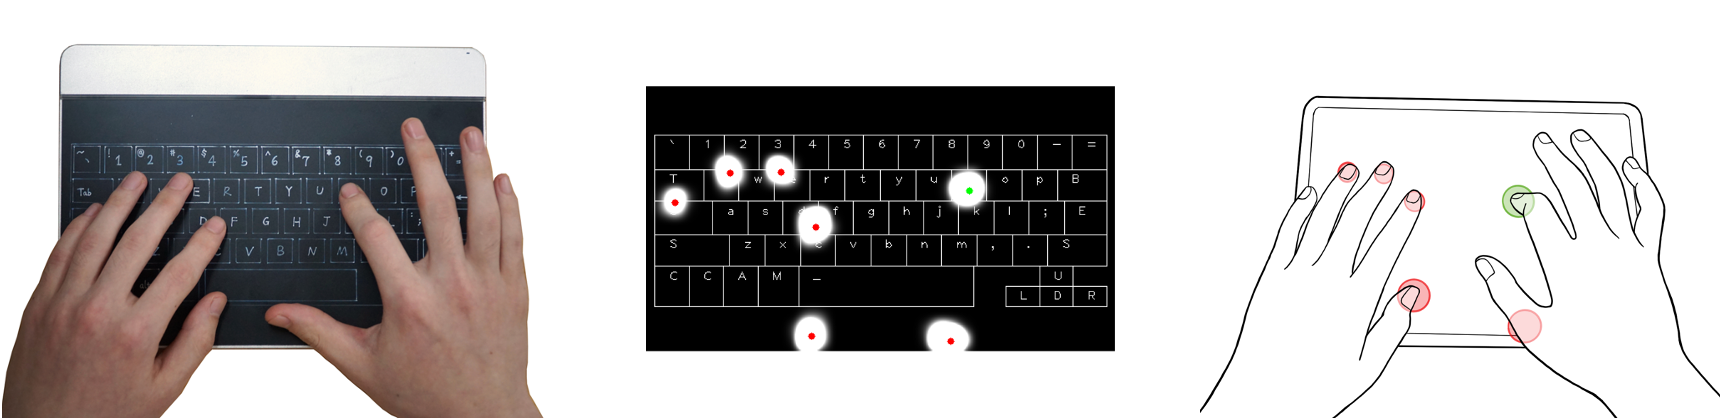
\includegraphics[width=\textwidth]{figures/TypeBoard_teaser.png}
	\caption*{TypeBoard是面向平板电脑文本输入的防误触技术,能够过滤文本输入中的误触(红色点),只对用户的打字触摸事件(绿色点)作出响应。}
	\caption{TypeBoard原理介绍}
	\label{fig:TypeBoard_teaser}
\end{figure*}

本文并不是第一份平板电脑文本输入的防误触工作。在2013,Kim等人就提出了TapBoard\cite{2013-TapBoard},这是一款从规则上自定义了有意和无意触摸的平板电脑文本输入技术,该技术将“敲击”视为有意的触摸交互,而将其它触摸行为都视为误触。“敲击”指的是触摸时长小于450毫秒且触摸期间手指位移小于15毫米的点击,在该规则的约束下,用户需要主动适应键盘才能正常打字,这导致了不自然的打字行为。而且,该技术必须在人的手指抬起时才能确定触摸的意图,并输入字母,相比之下,大多数文本输入技术都是在人的手指按下时就键入字母了。即便有以上种种约束,TapBoard的准确率也只有97\%。本章所介绍的TypeBoard有三条策略来克服先前工作的不足:首先,为了确保交互的自然性,本章从人的交互意图出发,将\textbf{误触}定义为不表达交互意图的触摸。第二,本章将通过用户实验来了解用户的打字行为,并据此设计更好的面向平板电脑的防误触技术。第三,本章将利用触摸运动模型,寻找能够有效区分有意触摸和无意触碰的特征。

上面提到,用户行为规律对技术的改进有帮助,但是反过来,技术也会改变用户行为。举例来说,用户不会在打字的时候将手指休息在触摸屏上,除非触摸屏拥有很强的防误触能力。在设计TypeBoard的过程中,研究者需要观察用户的打字行为,然而,最有价值的用户行为数据正是用户在TypeBoard上的打字行为数据。这就面临一个循环论证的问题:研究者如何在研发出TypeBoard之前观察并分析用户在TypeBoard上打字的行为呢?为了解决上述问题,本章采用迭代的实验方法来研该防误触技术,并先提出三个研究问题来理清这份工作的思路:\textbf{(RQ1)}用户在TypeBoard上的打字行为有何规律;\textbf{(RQ2)}如何基于用户打字行为设计TypeBoard防误触技术;\textbf{(RQ3)}用户使用TypeBoard打字的效率和体验如何?实验者组织了三个用户实验来回答以上研究问题。考虑到RQ1和RQ2是循环论证的,实验者采用迭代的实验方法来逼近这两个问题的答案:

\begin{enumerate}
	\item{\textbf{实验一:}\emph{用于回答RQ1和RQ2的第一轮迭代。}在实验一中,实验者收集了被试在没有反馈的触摸板上的打字数据。被试不能真正输入单词,而是想象可以输入单词,并且想象该触摸板能够防止所有误触。在这个实验中,实验者共观察到了11类误触行为,例如多指休息、小鱼际误触和边缘误触,等等。基于实验一的数据,实验者研发了\textbf{初版}TypeBoard。}
	\item{\textbf{研究二:}\emph{用于回答RQ1和RQ2的第二轮迭代。}在实验二中,实验者收集了被试在初版TypeBoard上的打字数据。结果显示,实验一中观察到的11类误触行为已经是误触类型的全集了,在实验二中未发现新的误触类型。然而,实验二的用户行为在细节上与实验一有一些差异。例如,在实验二中,有意触摸的平均压力减轻了33.78\%,这是因为在有反馈的情况下,被试们可以根据反馈用更轻的力气打字,以避免疲劳。基于实验二的数据,实验者研发了\textbf{终版}TypeBoard,防误触准确率达到了98.88\%,识别延迟为100毫秒。}
	\item{\textbf{研究三:}\emph{对TypeBoard进行评测,回答RQ3。}在实验三中,我们评测了被试在三种设置下的打字效率和用户体验,包括普通平板电脑软键盘、TypeBoard和TypeBoard+(有按键轮廓反馈的TypeBoard)。 结果表明,TypeBoard通过缓解疲劳问题、减轻认知负担、降低打字错误率大大提升了平板电脑上文本输入的效率和可以用性。TypeBoard+则是进一步的改进,让用户能够在平板电脑上盲打。}
\end{enumerate}

本章工作有三点主要贡献:首先,本章提出了面向平板电脑文本输入的防误触技术,简称TpyeBoard,能以98.88\%的准确率、100毫秒的延迟过滤触摸交互中的误触;第二,本章整理了平板电脑文本输入的用户打字行为;第三,本章通过用户实验证明,TypeBoard提升了平板电脑文本输入的交互体验,具体体现在打字效率、打字错误率和用户主观反馈三方面。

\section{相关工作}

\subsection{触摸交互中的防误触技术}

触摸交互是智能手机、平板电脑和智能大桌面等触摸屏设备的主要输入信道。并非所有触摸屏上的手指接触都应该触发数字响应,那些对用户的交互目标没有帮助的触摸被称为误触\cite{2020-TabletopTouch, 2015-GestureOn, matero2012identifying}。如果误触触发了不必要的数字响应,就会影响正常交互的效率和自然性\cite{2014-PenMightier, 2020-TabletopTouch}。不必要的数字响应会破坏用户的交互流程,用户需要花费额外的时间和操作来消除该响应的影响。随着时间的推移,用户会倾向于在屏幕屏设备上小心地进行触摸交互,以避免误触。例如,在普通的平板电脑上,用户打字时会将非交互手指悬停在触摸屏上,以避免误触,这种将手悬空的做法会导致疲劳问题\cite{2018-UbiK}。

尽管误触对交互有负面影响,但是误触在触摸屏交互中是不可避免的。例如,在人们日常使用智能手机的过程中,人手的大鱼际就会不断地触碰屏幕的边缘\cite{2018-PalmTouch}。幸运的是,各种各样的软件技术有机会过滤误触。在相关文献中,已经有广泛的工作致力于研究防误触算法,本节将通过两种分类方法来介绍相关工作:(1)应用场景,和(2)传感器类型。

\subsubsection{不同应用场景下的防误触技术}

在不同的应用场景下,误触的定义也会有所不同。若不对应用场景作出限制,误触指的是不表达交互意图的触摸\cite{2020-TabletopTouch};而在特定的交互任务中,误触的定义变得更加明确,例如,文本输入任务中的误触指的是不用于输入单词的触摸。

少量文献\cite{matero2012identifying, 2020-TabletopTouch}和大量专利\cite{2016-Classification,2006-PadUnint,2013-System,2013-Precluding,2015-TouchScreen}在不分应用场景的情况下识别误触。Metero等人整理了智能手机上的误触行为,并提出了智能手机上的防误触算法\cite{matero2012identifying},该方法能过滤79.6\%的误触。Xu等人利用眼动信号、头动信号和触摸屏触点信息识别触摸屏大桌面上的误触,准确率为91.3\%。上述方法的特点是适用于不同的应用场景,但是识别准确率较低。

在相关文献中,更多的实验致力于研究特定应用场景下的防误触问题。TapBoard\cite{2013-TapBoard}和TapBoard2\cite{2016-TapBoard2}在触摸屏文本输入任务下讨论误触问题。TapBoard将敲击手势识别为有意触摸,将其它所有触摸都识别成误触,其中,敲击手势指的是触摸时长小于450毫秒,触摸期间手指位移小于15毫米的触摸。用户需要主动适应技术中所规定额阈值来进行打字,这导致了不自然的用户行为。即便如此,TapBoard的误触识别率也只有97\%。TapBoard2进一步区分了打字触摸和用于目标选择的触摸,准确率为95\%。在基于触摸屏和电子笔的应用场景下,误触是最被诟病的问题之一\cite{2014-PenMightier},例如,在使用防误触能力有限的产品时,用户必须保持别扭的握笔姿势,以防止误触。有几份工作致力于研究电子笔场景下的防误触问题\cite{2013-PalmInput,2014-PenUnint,2014-PalmRejection}。Schwarz等人利用触摸的时空特征来训练误触过滤器,其准确率是同类型研究中最高的,能够将误触和有意交互的比例降低到0.016,同时正确识别98\%的有意交互。总体上来说,特定应用场景下的防误触技术准确率更高。

\subsubsection{不同传感技术下的防误触技术}

大量相关工作致力于研究触摸屏设备上的防误触方法,相关设备包括智能手机 \cite{matero2012identifying,2015-GestureOn,2018-PalmTouch,2019-BeyondUnint}、平板电脑\cite{2006-PadUnint,2014-PenUnint, 2014-PalmRejection, 2013-TapBoard, 2016-TapBoard2}和触摸屏大桌面\cite{2020-TabletopTouch}。大多数技术都仅利用触摸屏的触点信息\cite{matero2012identifying,2006-PadUnint,2014-PalmRejection,2013-TapBoard,2016-TapBoard2}和电容屏图像\cite{2018-PalmTouch,2014-PenUnint}。Metero等人利用触点信息识别智能手机触摸屏上的误触\cite{matero2012identifying}。他们提出了基于触摸时长、触摸位置分布和轨迹特征的误触过滤标准,成功过滤了79.6\%的误触,对有意触摸的未识别率仅为0.8\%。Schwarz等人提出了平板电脑上区分有意的电子笔输入和手掌误触的方法\cite{2014-PalmRejection},他们从触摸点中提取特征并使用决策森林训练机器学习模型。PalmTouch\cite{2018-PalmTouch}可以区分智能手机上的有意触摸和手掌误触,它利用触摸屏的电容图像作为输入,使用卷积神经网络(CNN)训练模型,在实测场景中达到了99.53\%的误触识别率。

另有一些工作通过增加传感能力来提高防误触能力\cite{2015-GestureOn,2020-TabletopTouch,2001-PalmPressure,2019-BeyondUnint}。GestureOn\cite{2015-GestureOn}能在智能手机处于待机模式的情况下区分有意的手势输入和误触,使得用户可以在打开屏幕之前通过手势触发快捷方式。GestureOn利用了绝大多数智能手机中的内置传感器,包括红外接近光传感器、惯性传感器、屏幕上的压力信号等等,通过多信号融合技术,GestureOn误触识别达到了98.2\%的精确率和97.6\%的召回率。Xu等人利用眼动信号、头动信号和触摸屏触点信息来识别触摸屏大桌面上的误触,结果表明,眼动信号和头动信号使得误触识别的准确率提升了4.3\%,达到达到91.3\%。总体来说,更多的传感信号的融合总是有利于提高防误触能力。

\subsubsection{小结}

本小节提出两个观点:首先,一般来说,防误触方法总是在场景受到限制的情况下效果更好。在特定场景下,有的防误触技术的准确率相当高,以至于让用户改变自身交互行为并从中收获更自然的交互体验\cite{2013-TapBoard,2016-TapBoard2,2014-PenMightier}。第二,多种传感信道的融合通常可以提高防误触能力。多项研究表明,额外的输入信道(例如压力信号 \cite{2015-GestureOn}、眼动和头动信号\cite{2020-TabletopTouch})有助于提高误触的识别率。在本章所述的面向平板电脑文本输入的防误触技术中,研究者也使用了压敏触摸屏,并将应用场景限定在文本输入交互任务中,在这两条前提下本技术应该能具备很强的防误触能力。

\subsection{触摸交互防误触技术的作用}

防误触技术的直接好处是降低误触对交互产生的负面影响,除此之外,本小节将防误触技术的其它用处总结如下。

\subsubsection{弥补触摸屏文本输入之于物理键盘的不足}

越来越多的人需要用到平板电脑的软键盘文本输入技术\cite{2018-Japanese},然而,平板电脑的软键盘在打字效率\cite{1991-Improving, findlater2011typing, 2010-Keyboard}和用户体验\cite{2014-Differences, lu2017blindtype, 2010-NoLook, 2010-Eyes}上无法与物理键盘相提并论。在物理键盘上,用户可以将手指休息在键帽上,这是物理键盘的重要特性:首先,这可以缓解长时间打字的疲劳问题\cite{2013-TapBoard};第二,用户通过触摸键帽的轮廓来定位自己的手指位置,从而通过盲打提高打字效率\cite{2010-Warning, 1995-Use, 2011-Hierarchical, 2015-Haptic}。在平板电脑的软键盘上,若能实现一种强大的防误触技术,使得用户能在打字时将非交互手指休息在触摸屏上,将能显著缓解疲劳问题。更进一步地,在手指休息不会触发不必要的误触的前提下,研究者可以通过可变形触摸屏\cite{Website-Tactus}或可变触摸屏纹理技术\cite{2011-Stimtac, 2010-TeslaTouch, 2011-Enhancing}来模拟物理键盘上键帽的触觉反馈,从而使得用户在平板电脑上也能盲打。如此一来,触摸屏软键盘和物理键盘之间的差距就会缩小。

\subsubsection{将误触输入作为有用的交互信息}

大部分与误触相关的工作的目标都是去除误触,然而,一部分试图将误触应用于情景感知\cite{2019-PenTouch}和有意交互\cite{2017-HandContact, 2018-PalmTouch, 2016-TapBoard2}。手掌在平板电脑上的按压通常被视为误触,但Zhang等人手掌按压作为平板电脑上一种新的触发命令的方式\cite{2019-PenTouch},增强了平板电脑上的电子笔交互。例如,当用户在用电子笔绘画时将手掌按压在屏幕上,在手掌周围就会出现一圈绘画工具,方便用户的使用。前臂本是触摸屏大桌面的典型误触部位,但Koura等人将前臂的触碰应用于触摸屏大桌面的菜单操作中\cite{2012-Amazing}。Matulic等人将各种手掌与触摸屏的接触姿态用于丰富触摸屏大桌面的交互,该系统以91\%的准确度分类七种不同的接触姿态,可用于触发和控制菜单和小工具部件。PalmTouch可以区分手指触摸和手掌触摸,并将手掌触摸定义为一种快捷触发方式\cite{2018-PalmTouch}。TapBoard2可以区分打字和普通触摸行为\cite{2006-TouchType},从而统一了软键盘和触摸板的空间,省去了用户在不同设备之间来回切换的成本。

\section{初版防误触键盘}

\subsection{实验一:收集无反馈键盘上的打字数据}

实验一采集了用户在一块压敏触摸板上的打字数据,这一实验是探索用户在TypeBoard上打字行为的第一轮迭代,研究用户打字行为有助于防误触技术的设计,基于本实验的数据本节将介绍\textbf{初版防误触键盘}技术。由于(不正确)的反馈可能会影响用户的行为,在这个实验者,被试们在无反馈的条件下打字:被试们并非真的输入单词,而是想象他们的打字行为能够输入单词,同时,被试需要想象该触摸板能够完美地防止误触。

\subsubsection{被试}

实验者从校园中要求了16名被试参与实验,实验者的年龄从19岁到26岁不等,平均年龄22.13岁,标准差为2.13,其中,有8名女性被试。所有被试都是右撇子,他们使用智能手机触摸屏文本输入的时间不少于两年,平均7.50年,标准差为2.25。所有用户都有物理键盘打字经验,有8名被试有使用平板电脑打字的经验。

\subsubsection{实验设备}

如图\ref{fig:TypeBoard_study1_illu}所示是实验设置,实验者将微软的Surface平板电脑和Sensel压敏触摸板\cite{Website-Morph}拼在一起,以代替还未商业化的压敏触摸显示屏。压敏触摸板包含185$\times$105个传感元件,间距为1.25毫米。每个传感单元可以感应到大约30000个级别的压力,范围从5克到5千克不等。压敏触摸板提供压力图像和触摸点信息,包括触摸点的位置、时间戳、面积、压力和拟合椭圆的参数。压敏触摸板的感应区域大小为240毫米$\times$138毫米。实验者使用荧光笔在触摸板上手工绘制了二十六键键盘布局,以模拟触摸显示屏上的键盘布局。由于压敏触摸板的宽度(240毫米)比典型笔记本电脑(15英寸苹果电脑)上的键盘宽度(270 毫米)小。实验者在绘制键盘布局时移除了一些不常用的按键,例如方括号和分号,如此一来,二十六键键盘的布局就可以完整地绘制在压敏触摸板上了,而每个按键的大小与苹果电脑保持一致(17毫米)。平板电脑是微软Surface Pro6,装配i7英特尔酷睿处理器。实验所用的程序以50赫兹运行。

\subsubsection{实验设计和过程}

\begin{figure}[!tbh]
	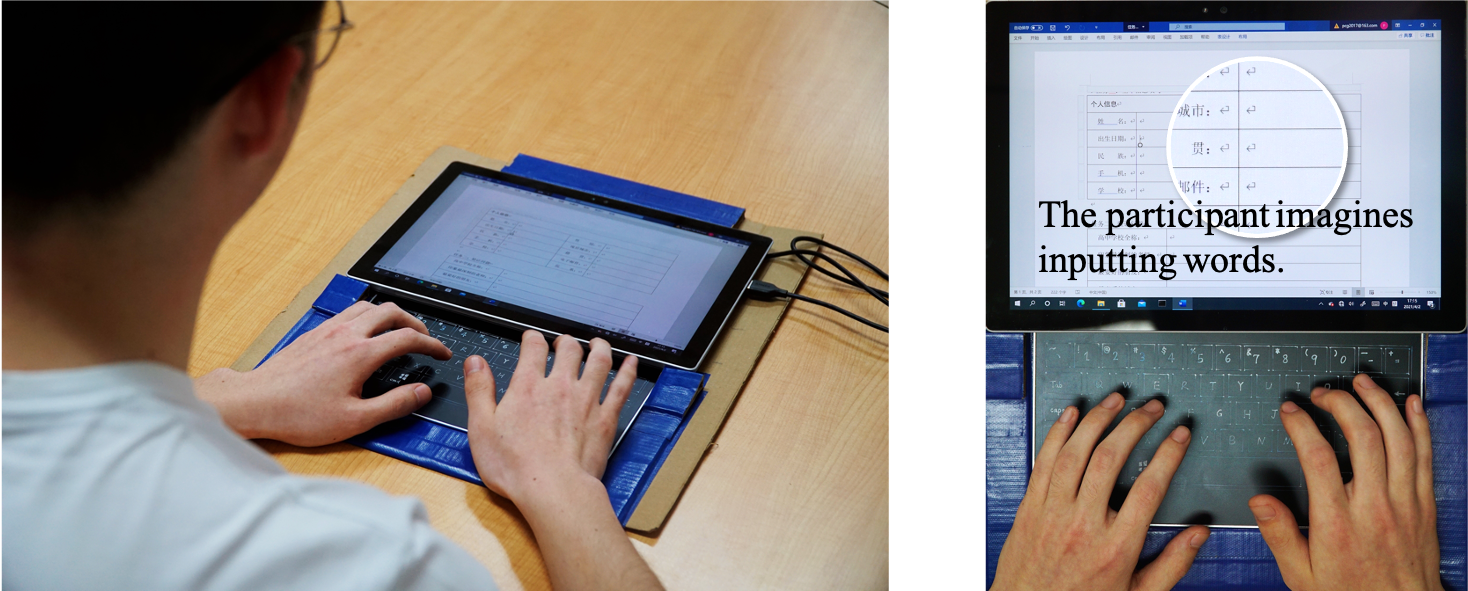
\includegraphics[width=1.0\linewidth]{figures/TypeBoard_study1_illu.png}
	\centering
	\caption*{实验者将一个平板电脑和一个压敏触摸板拼接在一起,以模拟带有压敏触摸屏的平板电脑。被试在无反馈的情况下想象在平板电脑上打字。}
	\caption{实验一的实验设置}
	\label{fig:TypeBoard_study1_illu}
\end{figure}

实验任务是一份填写一份Word表格,该表格显示在平板电脑上。被试通过平板电脑上的触摸交互来选择表格中的单元格,通过在Sensel压敏触摸板上连续触摸点击来想象打字的情景。被试需要按照实验任务做出打字的动作,只是平板电脑不会对打字动作作出反馈。实验表格包含四个任务:(1)填写个人信息;(2)简短的问题;(3)模拟开卷考试;(4)看图写话。实验语言为中文。实验通过拉丁方来平衡以上四个任务的出场顺序。与典型的文本输入相关文献\cite{2003-Metrics, mackenzie2003phrase, 2017-Word}不同,本实验未包含誊写任务,这是因为实验者通过预实验发现,在誊写任务中被试很少会将手指休息在触摸屏上,因此誊写任务将不利于误触数据的收集。

\begin{enumerate}
	\item \textbf{填写个人信息}:实验表格中有十个空的单元格属于填写个人信息任务,填写的内容包括姓名、性别等等。如图\ref{fig:TypeBoard_study1_task}(a)所示是个人信息任务的图例和英文翻译。这一项实验任务代表那些需要频繁切换文本输入和光标控制的交互任务。为了保护被试的隐私,被试们可以在表格中填入虚构的个人信息,前提是他们需要记得自己填了什么,因为记得所填写的内容对后续的人工标注过程至关重要。
	\item \textbf{简单的问题}:实验表格中包含十个简短的问题,例如“你最喜爱的颜色是?”、“你最好的朋友是?”。同样地,为保护被试的隐私,被试可以在表格中给出虚构的回答。
	\item \textbf{模拟开卷考试}:实验表格中的模拟开卷考试部分包含五个很难的问题,例如,“元素周期表中第50号元素是什么?”。被试很有可能不知道问题的答案,因此他们需要使用搜索引擎搜索答案。在本实验中,被试只是想象打字,他们边做出打字的动作边将打字内容说出来,实验者代替他们在浏览器中搜索相关内容。这一项实验任务代表需要浏览网页的一类交互任务。
	\item \textbf{看图写话}:如图\ref{fig:TypeBoard_study1_task}(b)所示,被试通过五句话来描述图中的场景。被试边做出打字的动作边将打字内容说出来,实验者代替他们输入文字。这一项实验任务代表自由写作这一类交互任务。
\end{enumerate}

\begin{figure}[!tbh]
	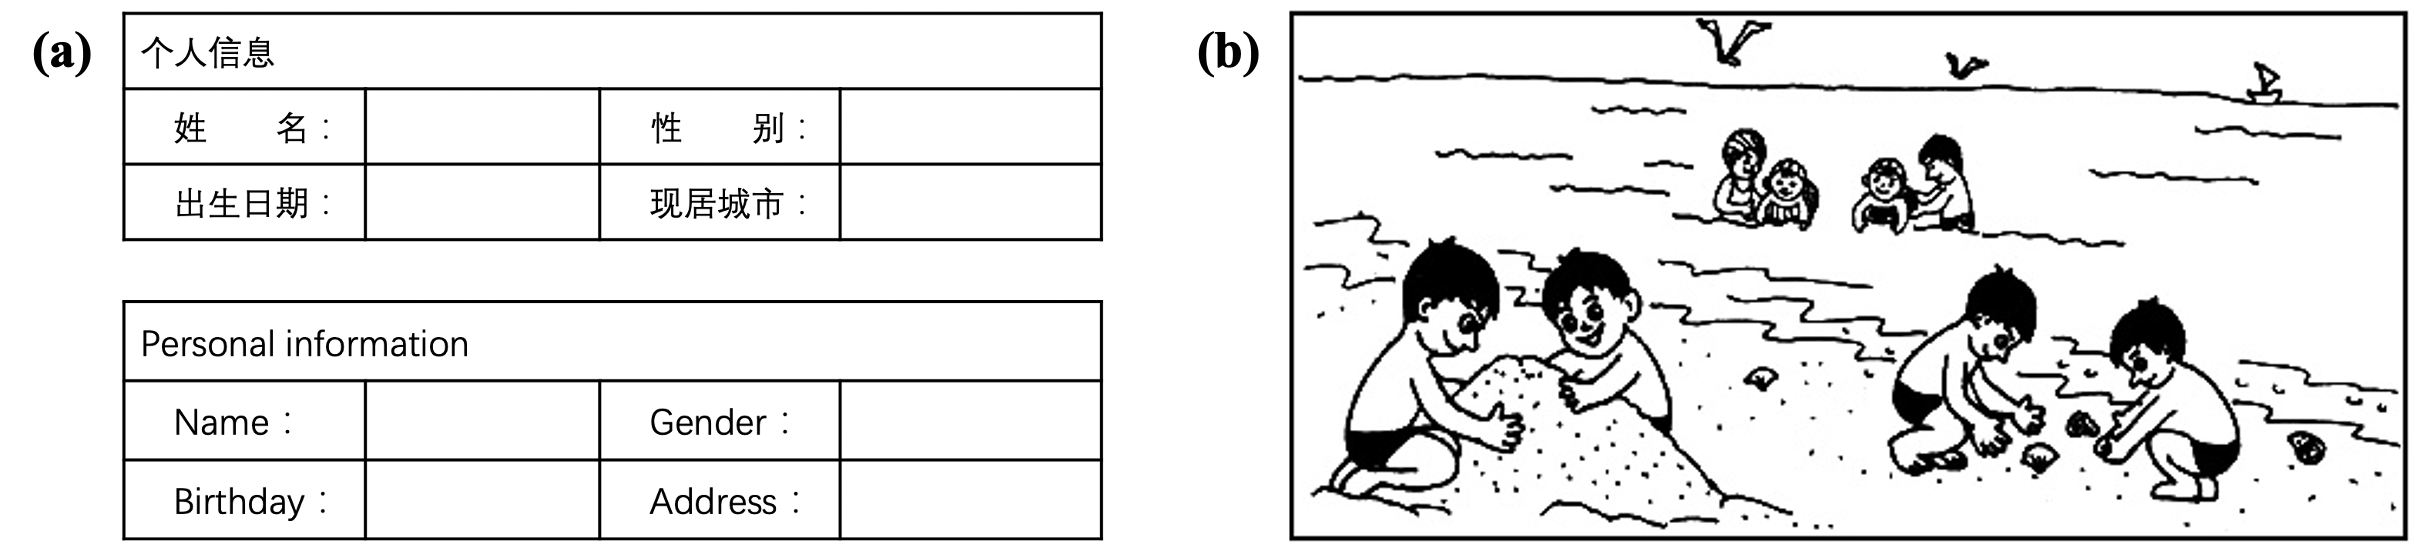
\includegraphics[width=1.0\linewidth]{figures/TypeBoard_study1_task.png}
	\centering
	\caption*{如图所示是实验表格中的任务。左侧是填写个人信息部分的内容,右侧是看图写话部分的内容。}
	\caption{实验任务图示}
	\label{fig:TypeBoard_study1_task}
\end{figure}

在正式实验开始之前,被试有五分钟的练习时间熟悉实验流程。在练习阶段,被试可以在触摸板上自由打字,打字过程没有反馈。在被试自由练习的过程中,实验者会提醒被试两点注意事项。首先,触摸板上的键盘没有任何反馈,被试不能真的输入文本,而只是做出打字动作,想象文本被成功输入。第二,被试需要想象该触摸板键盘能够过滤所有的误触,并据此改变自己的打字行为,例如,当被试在思考打字内容的时候可以将手指休息在触摸板上。

\begin{figure}[!tbh]
	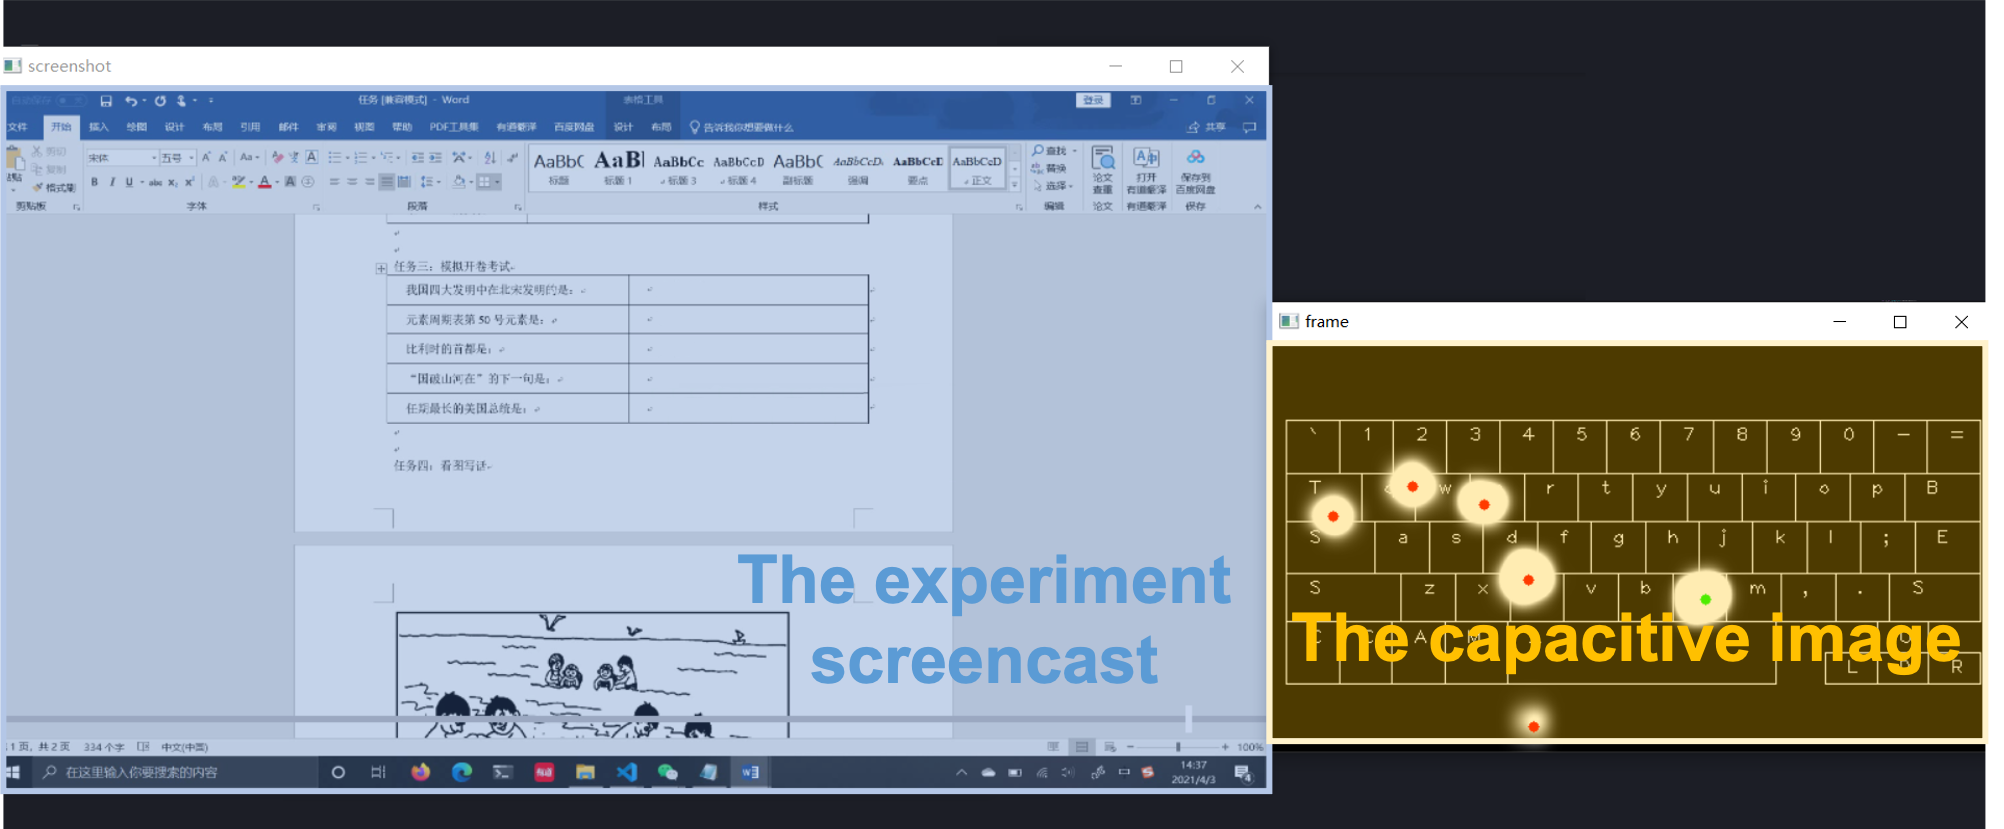
\includegraphics[width=1.0\linewidth]{figures/TypeBoard_label_process.png}
	\centering
	\caption*{如图所示是人工标注过程中显示器中的内容。左侧是实验录屏,右侧是触摸板记录的触点数据的可视化,被试在右侧的可视化程序中给触点的有意性做人工标注。}
	\caption{标注程序图示}
	\label{fig:TypeBoard_label_process}
\end{figure}

在每一项实验任务之后,被试都会给刚刚实验中触点的有意性做人工标注。如图\ref{fig:TypeBoard_label_process}所示,被试通过一个交互式程序给触点数据进行标注,程序既展示了实验过程中的录屏,也展示了触点数据的可视化图像,两个图像的时间轴是对齐的。可视化图像上的每个红色点表示一个触点,被试通过回忆来把其中的有意触摸标记成绿色。如果被试忘记了某个触点的有意性,可以将触点标记成蓝色,表示删除该数据。这个人工标注的准确性是可以保证的,因为被试可以通过实验录屏中的上下文信息来帮助回忆。平均而言,被试总共花10分钟的时间来完成实验表格中的内容,花45分钟的时间来给实验收集的触点数据做人工标注,被试在每两项实验任务之间都会休息5分钟的时间,因此实验的总时长约为70分钟。

\subsection{基于打字行为设计初版防误触键盘}\label{section:model_TypeBoard}

本实验收集的数据集包含12659个触点,不包括人工标注中被剔除的数据点。数据集包含67.5\%的有意点击样本和32.5\%的误触样本。基于该数据集,实验者分三个阶段研发了初版TypeBoard防误触技术,该技术基于支持向量机。如表格\ref{tab:TypeBoard_study_features}所示是防误触技术的总览,展示了该技术的三个阶段中所涉及的机器学习特征和测试准确率。每一个特征组都是针对一种或者多种有意性容易混淆的情形而设计的,可以直接提升误触识别的准确率。本小节的剩余内容将分三个阶段详细介绍防误触技术的研发过程。

\begin{table}[!tbh]
	\centering
	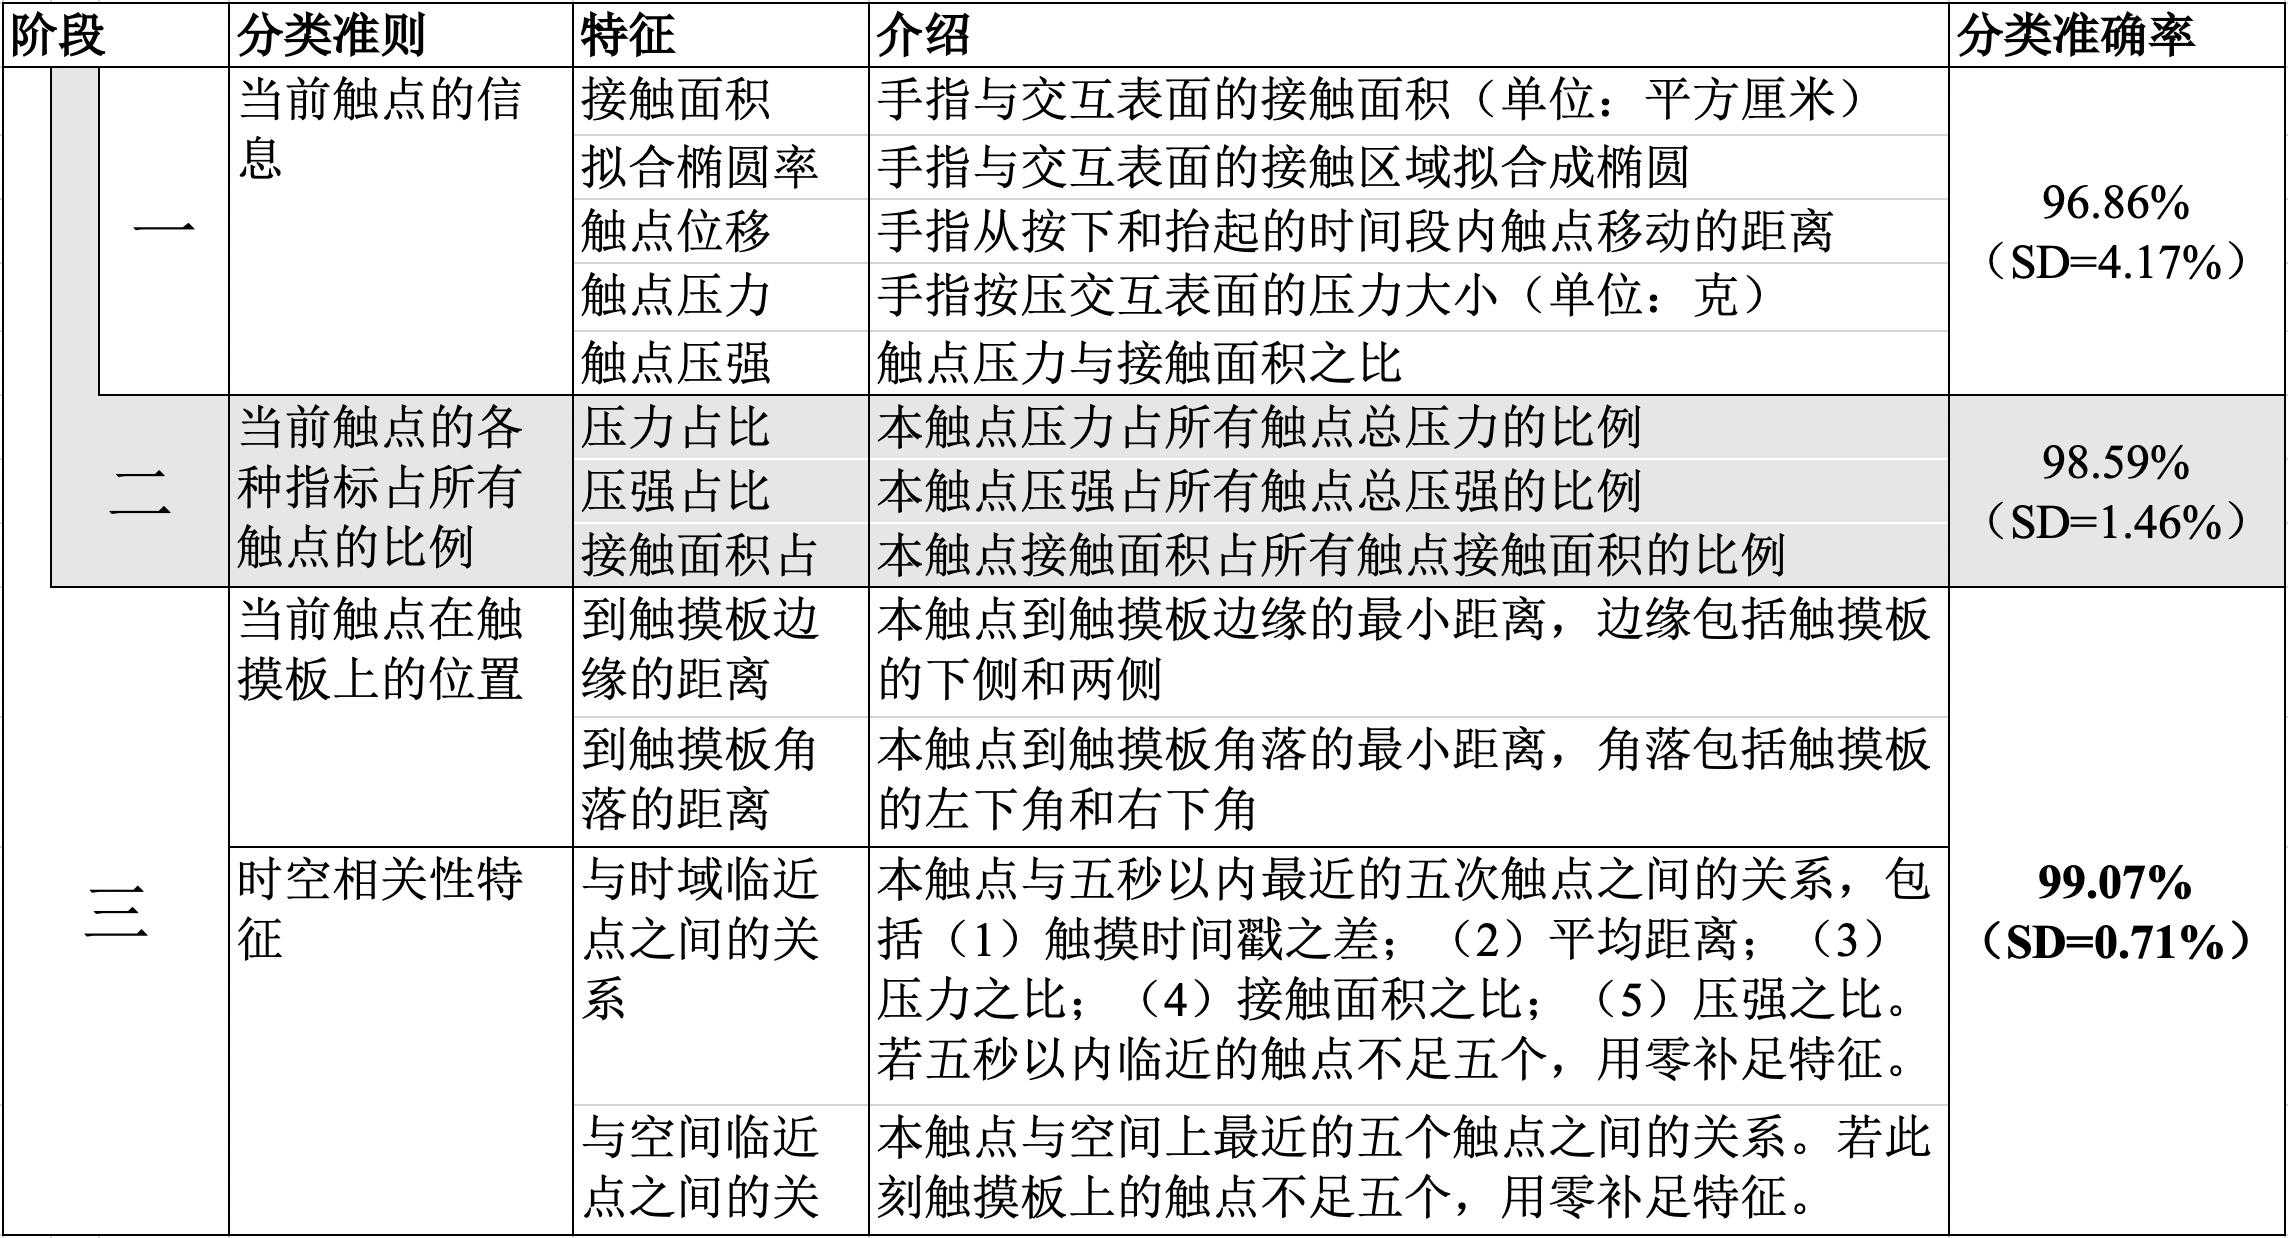
\includegraphics[width=1.0\linewidth]{figures/TypeBoard_features.png}
	\caption{表格中展示了三个阶段中喂入支持向量机模型的特征组。除了“时空相关性特征”以外,其余特征组都需要提取100毫秒内的时域特征,包括最大值、最小值、平均值、峰度和偏度。}
	\label{tab:TypeBoard_study_features}
\end{table}

\subsubsection{阶段一:用简单模型检查标注效果}

由于一些被试误解了误触的概念,数据集中存在一些被错误标记的触摸点。实验者通过简单的特征提取来训练一个简单的模型,并使用该模型来负荷人工标注的结果。实验者对每次触摸事件后的连续五帧(100毫秒)进行采样,如果触摸持续时间短于五帧,则对整个手指接触交互表面的过程进行采样。如表格\ref{tab:TypeBoard_study_features}(阶段一)所示d,实验者从样本中提取了如下特征:对于手指接触面积、拟合椭圆的椭圆率、位移、按压力度和压强,计算时域特征,包括五帧中最大值、最小值、平均值、偏度和峰度,然后将这些值拼接起来,得到一个25维的特征向量,喂入支持向量机中训练识别误触的二分类模型。这就是阶段一的防误触技术。

实验者用该模型来对数据集中每一个触点的有意性进行分类,发现其中一部分被试误解了误触的概念,例如,将打字过程中打错字母的情况也算成误触了。实验者通过电子邮件要求被试重新标注这些可疑的数据点。至此,实验者认为数据的标注是真正可靠的了,因为数据标注经过了被试、实验者和简单分类模型的三重校验。校验过后还剩下12624个数据点,包括68.38\%的有意触摸样本和31.62\%的误触样本。留一(被试)交叉验证表明,阶段一防误触技术的准确率为96.86\%(SD=4.17\%)。

\subsubsection{阶段二:过滤多指休息行为导致的误触}

实验数据分析发现,大部分误触来自被试的多指休息行为,这种行为导致的误触占误触总量的72.66\%。在本实验中,实验者告知被试,应当想象该触摸板具有完美的防误触能力。在此背景下,被试的确会在打字过程中将手指休息在触摸板上,以避免疲劳。由于被试将手指休息在触摸板上的行为并不表达打字的意图,因此这些手指接触交互表面时带来的触点都属于误触,应该被防误触算法过滤。在这样的用户打字行为之下,过滤多指休息行为导致的误触问题就变得尤为关键。如表格\ref{tab:TypeBoard_study_features}(阶段二)所示,实验者添加了一类触摸意图分类准则(占比),用于过滤多指休息行为导致的误触。在多指休息行为中,手指往往是陆续接触到交互表面的。在大部分情况下,在第一根手指触摸之后,后续的手指会在100毫秒以内接触交互表面:在86.05\%的样本中,第二根手指会在100毫秒以内接触交互表面;在76.30\%的样本中,第二、第三根手指都会在100毫秒以内接触交互表面。由于本模型的考虑触摸发生后五帧的数据,识别延迟为100毫秒,该模型有很大的机会来正确识别一次多指休息行为,从而将这些触摸点判定为误触。如表格所示,实验者添加了三个特征组来过滤多指休息行为导致的误触,这三个特征组分别对应触点的压力、压强和接触面积占此刻所有触点的相应属性之和的比例,对占比求时域特征即得到特征组。留一(被试)交叉表明,阶段二防误触技术将误触的识别准确率提升至98.59\%(SD=1.46\%)。实验者用两种指标来衡量该防误触技术的错误率:(1)假正率——将一次误触识别成有意触摸的概率;(2)假负率——将一次有意触摸识别成误触的概率。本防误触技术的假正率为3.16\%,假负率为0.59\%。

\subsubsection{阶段三:理解用户打字行为并深入改进技术}

实验者通过分析阶段二防误触技术中预测失败的案例来理解用户打字行为中容易导致误触的部分,从而指引防误触技术的改进方向。如表格\ref{tab:TypeBoard_fail_cases}所示,实验者将预测失败的案例分为16类,包括十种容易误触的情况,和六种容易被识别为误触的有意触摸。实验者对每一类预测失败的案例进行计数,讨论其原因,并给出可能的解决方案。对于表格中白色部分的触摸案例,实验者认为机器有能力正确识别其有意性,对于这些案例,实验者提出了新的特征组来提升模型的预测准确率。下面是一些例子:

\begin{enumerate}
	\item \textbf{例一}:\emph{小鱼际误触}。如图\ref{fig:TypeBoard_fail_case_examples}(a) 所示,小鱼际指的是控制小指运动的肌肉群,而大鱼际指的是在拇指根部上的肌肉群。大鱼际误触和小鱼际误触都是触摸交互中常见的误触类型。而在平板电脑十指打字这一交互任务下,小鱼际误触更是十分常见,这是因为在十指打字过程中小鱼际经常会以较大的力度触碰到触摸屏,这很容易引起误触。幸运的是,小鱼际误触总是出现在触摸板的左下角或者右下角,因此,“与触摸板四个角的距离”这一数值成为过滤小鱼际误触的有效特征。
	\item \textbf{例二}:\emph{连续触摸}。当一名被试连续触摸键盘上的同一按键(如删除键)时,从第二次触摸开始点击的力度会变得更轻(p<.005)。实验数据分析表面,在对同一个按键的连续触摸中,第一次触摸的平均力度为167.01克(SD=106.76),而后续触摸的平均力度为150.42克(SD=112.70)。由于后续触摸更轻,它们更有可能被误识别为误触,因此时域上临近触点的信息将有利于对触摸有意性的判断。
	\item \textbf{例三}:\emph{单手打字}。如图\ref{fig:TypeBoard_fail_case_examples}(b)所示,有时候被试会用单手打字,另一只手休息在触摸屏上。在这种情况下,阶段二的防误触算法可能会认为此刻所有的触点都是多种休息行为导致的误触,但实际上正在打字的手指所触发的是有意触摸。由于打字手指和休息中手指之间距离往往比较远,因此空间上临近触点的信息将有利于对触摸有意性的判断。
\end{enumerate}

\begin{figure}[!tbh]
	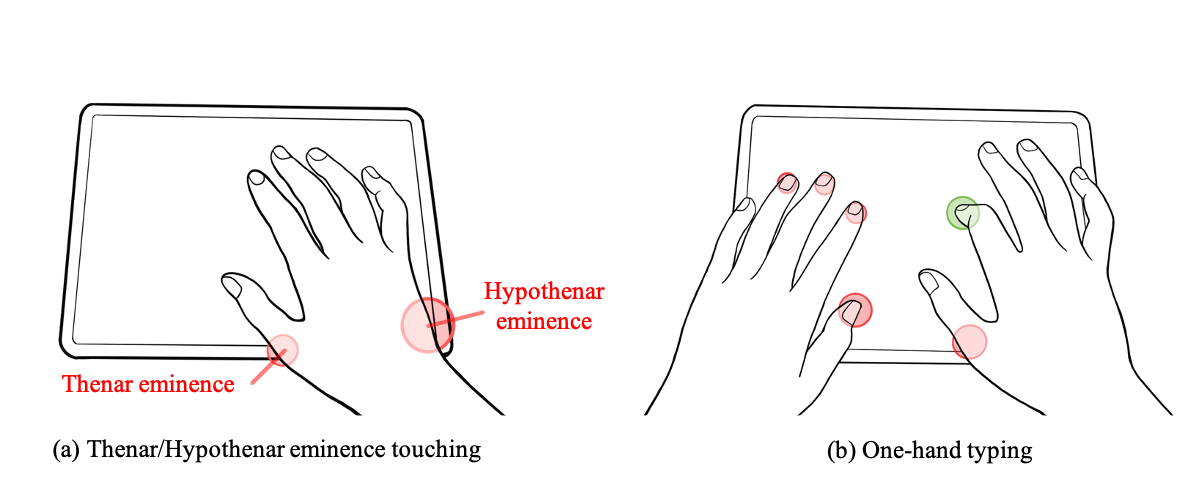
\includegraphics[width=1.0\linewidth]{figures/TypeBoard_fail_case_examples.png}
	\centering
	\caption*{左图展示了小鱼际误触和大鱼际误触,右图展示了一手打字、一手休息的情况。}
	\caption{有意性易混淆的案例}
	\label{fig:TypeBoard_fail_case_examples}
\end{figure}

\begin{table*}[htbp]
	\centering
	\begin{tabular}{|p{6.4em}|p{16em}|r|p{10em}|}
		\toprule
		\textbf{案例} & \textbf{介绍} & {\textbf{N}} & \textbf{有用的特征} \\
		\midrule
		\multicolumn{4}{|l|}{\textbf{假正(容易被识别成有意触摸的误触)}} \\
		\midrule
		小鱼际误触 & 如图\ref{fig:TypeBoard_fail_case_examples}(a)所示 & 23    & 触点位置,与触摸板角落的距离 \\
		\midrule
		大鱼际误触 & 如图\ref{fig:TypeBoard_fail_case_examples}(a)所示 & 2     & 触点位置,与触摸板边缘的距离 \\
		\midrule
		时域重复报点 & 一次触摸被系统汇报了两次 & 12    & 时域临近点的信息 \\
		\midrule
		空间重复报点 & 一次触摸被系统识别成了两个触点 & 3     & 空间临近点的信息 \\
		\midrule
		边缘误触 & 用户在抓握设备时常有的误触 & 7     & 触点位置,与触摸板边缘的距离 \\
		\midrule
		二指休息 & 两只手指休息在屏幕上 & 3     & 空间临近点的信息 \\
		\midrule
		轻触误触 & 输入单词时多出来的一次轻轻的点击 & 9     & 该触点是否比最近的触点更轻 \\
		\midrule
		滑动误触 & 滑动通常不表达打字意图 & 7     & 触点的位移 \\
		\midrule
		\rowcolor[rgb]{ .949,  .949,  .949} 单指休息 & 两只手指休息在屏幕上 & 9     & \textbf{无解} \\
		\midrule
		\rowcolor[rgb]{ .949,  .949,  .949} 重触误触 & 输入单词时多出来的一次较重的点击 & 15    & \textbf{无解} \\
		\midrule
		\multicolumn{4}{|l|}{\textbf{假负(容易被识别成误触的有意触摸)}} \\
		\midrule
		连续触摸 & 连续点击同一个按键时,后续点击变轻 & 13    & 时域临近点的信息 \\
		\midrule
		粘滞打字\cite{2018-Observations} & 在前一只手指抬起之前,下一只手指已按下 & 12    & 时域临近点的信息 \\
		\midrule
		单手打字 & 一只手打字,另一只手多指休息 & 6     & 空间临近点的信息 \\
		\midrule
		手掌触摸 & 一只手指打字的同时,手掌造成了多个误触点 & 5     & 空间临近点的信息 \\
		\midrule
		\rowcolor[rgb]{ .949,  .949,  .949} 轻触触摸 & 很轻但有意的触摸 & 46    & \textbf{无解} \\
		\midrule
		\rowcolor[rgb]{ .949,  .949,  .949} 小面积触摸 & 触摸面积很小但有意的触摸 & 6     & \textbf{无解} \\
		\bottomrule
	\end{tabular}%
	\caption{阶段二防误触算法的预测失败案例,N表示失败案例计数。}
	\label{tab:TypeBoard_fail_cases}%
\end{table*}%

然而,对于表格\ref{tab:TypeBoard_fail_cases}中灰色部分的触摸案例,即使是人类(实验者)也无法在不观察实验录屏的情况下区分其有意性。实验者任务,这部分触摸案例被误识别是无法避免的。这里有一些例子:第一,极少数情况下被试会将一只手指重重地休息在触摸板上,这一类误触会与有意触摸混淆;第二,在被试输入一个单词的过程中,有时候点击其中一个字母的力度极轻,这一类有意触摸会与误触混淆。因此,根据对表格中灰色部分触摸案例的计数,实验者认为,防误触技术在本数据集上存在一个准确率的理论上限,约为99.40\%。

根据表格\ref{tab:TypeBoard_fail_cases}中汇总的有意性易混淆的触摸案例,实验者进一步添加了两条触摸意图分类准则,形成阶段三的防误触技术。第一条分类准则与触点的位置有关,包括触点距离边缘和角落的最短距离。实验者并未将触点位置与二十六键键盘布局的关系考虑进去,这是因为触摸屏上软键盘的布局是可以变化的,而实验者希望得到的是一个与键盘布局解耦的通用化防误触算法。第二条分类准则是连续触摸的时空相关性特征,包括本触点与时域临近点之间的关系,和本触点与空间临近点之间的关系。具体的特征描述在表格\ref{tab:TypeBoard_study_features}(阶段三)中。阶段三防误触算法用到表格中的所有特征,拼接起来形成刚好100维的特征向量,喂入支持向量机中训练识别误触的二分类模型。留一(被试)交叉验证显示,误触识别的准确率为99.07\%,假正率为1.77\%,假负率为0.54\%。至此,实验者已经得到了一个高准确率的误触识别分类器。然而,正如本章在引言中所述,实验一所采集的用户打字行为数据并不能完全代表用户在强力防误触键盘上的打字行为,因此,实验者将阶段三的防误触技术命名为初版TypeBoard。下一个实验将采集被试在初版TypeBoard上的打字行为数据,并使用新的数据来改进技术。

\section{终版防误触键盘}

\subsection{实验二:收集初版防误触键盘上的打字数据}

实验二收集了被试在初版防误触键盘上的打字行为数据,其中,初版防误触键盘是基于实验一数据的技术。实验二是探索用户在TypeBoard上打字行为第二轮迭代,研究该用户行为有助于防误触技术的改进,基于实验数据本节将介绍\textbf{终版防误触键盘}技术。

\subsubsection{被试}

实验者从大学校园中邀请了16名被试参与实验,被试年龄从19岁到37岁不等,平均年龄为22.19岁,标准差为4.55,有6名女性被试。所有被试都是右撇子,没有参加过先前的用户实验。被试们都至少有一年的智能手机软键盘输入法使用经验,平均经验为5.88年,标准差为2.36。10名被试曾经使用过平板电脑上的文本输入法。

\subsubsection{实验设计和过程}

如图\ref{fig:TypeBoard_study2_illu}所示,实验设备包括一台微软Surface平板电脑、一块Sensel压敏触摸板和一副耳机。实验共包含四项实验任务,任务与实验一相同,分别是在实验表格上填写个人信息、回答简单的问题、模拟开卷考试和看图写话。实验二与实验一的不同点是:(1)被试可以通过防误触键盘打字,而不是像实验一中一样只能在无反馈的键盘上做打字动作;(2)键盘具有一定的防误触能力,初版防误触键盘技术能够过滤大部分误触。在实验中,被触摸板判定为有意的触摸都会触发输入法响应,并有声音反馈,而被触摸板判定为误触的触摸不会引发任何响应。

\begin{figure}[!tbh]
	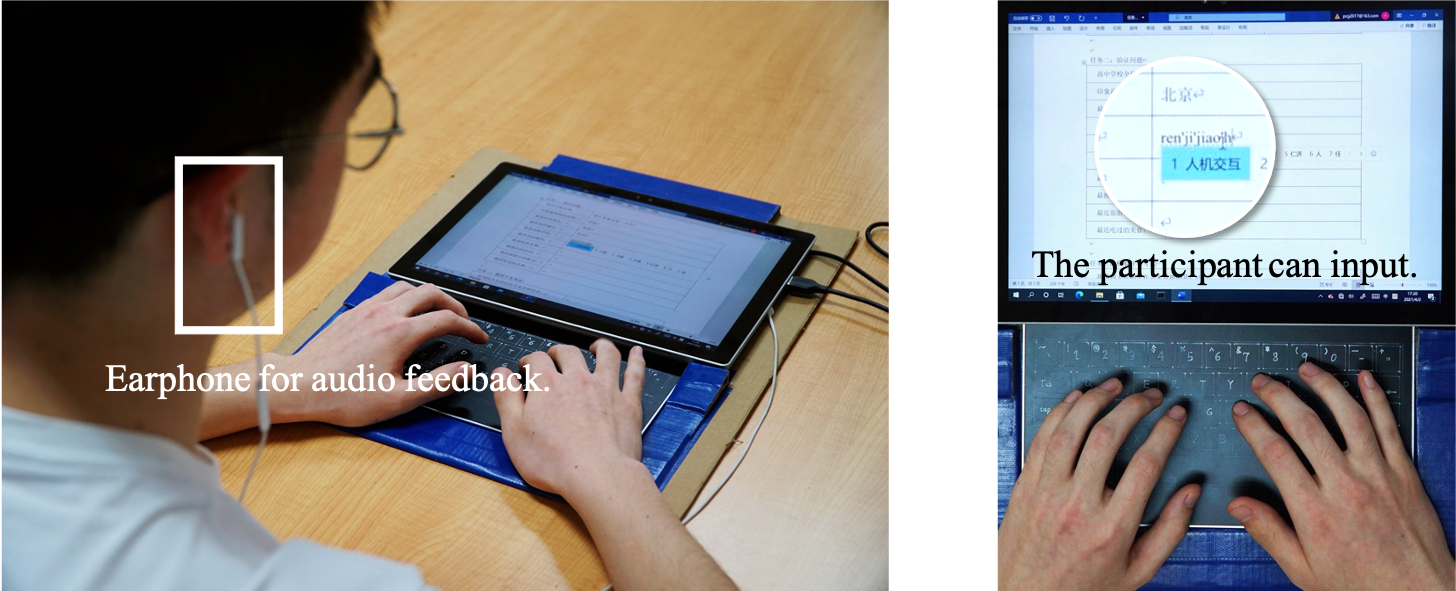
\includegraphics[width=1.0\linewidth]{figures/TypeBoard_study2_illu.png}
	\centering
	\caption*{实验二的设备包括一台平板电脑、一块压敏触摸板和一副耳机。}
	\caption{实验二的实验设置}
	\label{fig:TypeBoard_study2_illu}
\end{figure}

在正式实验之前,被试有五分钟的时间通过自由打字来熟悉实验设置。由于所有被试都没有在强力防误触触摸屏键盘上打字的经验,实验者提醒被试留意,在打字过程中可以将非交互手指休息在键盘上。被试可以根据自己的个人喜好和打字状态选择休息或不休息手指。在每项实验任务之后,被试像实验一一样标注每个触点的有意性。平均而言,每名被试总共花15分钟在文本输入任务上,花一个小时在数据标注上。在每两项实验任务之间,被试休息五分钟的时间,以避免疲劳。整个用户实验用时90分钟,时间比实验一长,这是因为在实验二中被试需要真正输入文本,选词和纠错消耗了更多的时间。

\subsection{基于打字行为设计终版防误触键盘}

排除了标注过程中无法辨认有意性的触点后,实验数据共包含13789个触点,其中包含71.01\%的有意触摸和28.99\%的误触。实验一之后训练得的初版防误触技术在实验二的数据集下准确率为98.05\%(SD=1.51\%),假正率为1.35\%(SD=1.28\%),假负率为2.20\%(SD=1.93\%)。初版防误触技术在实验二中的准确率与在实验一中的准确率相比,下滑了一个百分点,这说明实验一采集的数据和实验二采集的数据之间存在差异。由于实验二的实验设置更接近真实场景,本小节有必要将两个实验中的数据差异讨论清楚。

与实验一相比,实验者并未发现新的误触行为类型。然而,在用户行为细节上两个实验的数据存在差异。表格\ref{tab:behavior_difference}中举起了一些例子。首先,实验二中被试的触摸力度比显著比在实验一中的更轻($t_{15}=-2.78, p<.01$),在实验二中,被试是在有反馈的环境下打字的,当他们发现更轻的触摸依然能够成功触发输入法的响应后,便会逐渐减轻按键的力度,以节省体力。第二,在实验二的数据中,存在更多连续触摸的情况($t_{15}=3.57, p<.005$),即连续两次触摸之间的位移小于0.5个按键宽度、时间间隔小于500毫秒。这一现象主要是因为在是实验二中,被试需要连续点击退格键来删除错误的单词。第三,实验二数据中的粘滞打字现象更为少见($t_{15}=-6.32, p<.001$)。粘滞打字现象指的是在前一只手指抬起之前,下一只手指已经按下。在实验二中,被试的打字动作更慢,因此粘滞打字现象会减少\cite{2018-Observations}。

\begin{table*}[htbp]
	\centering
	\begin{tabular}{|p{4em}|p{8em}|p{4.8em}|p{4.8em}|p{3em}|p{6em}|}
		\toprule
		\textbf{量} & \textbf{介绍} & \textbf{实验一} & \textbf{实验二} & \textbf{Levene} & \textbf{T检验} \\
		\toprule
		触摸压力 & 有意触摸的平均压力 & 188.39g SD=64.72 & 124.75g SD=60.71 & 拒绝 & $t_{15}=-2.78$, $p<.01$ \\
		\midrule
		连续触摸 & 连续触摸数量占有意触摸的比例 & 4.02\% SD=1.96\% & 11.89\% SD=4.41\% & 通过  & $t_{15}=3.57$, $p<.005$ \\
		\midrule
		粘滞打字 & 粘滞打字数量占有意触摸的比例 & 17.60\% SD=9.34\% & 7.73\% SD=5.22\% & 通过  & $t_{15}=-6.32$, $p<.001$ \\
		\toprule
	\end{tabular}%
	\caption{实验一和实验二之间的用户打字行为差异。本节用T检验来评估差异的显著性,如果Levene测试拒绝了数据的同方差性,本节将使用不等方差T检验来代替T检验。}
	\label{tab:behavior_difference}%
\end{table*}%

如图\ref{fig:TypeBoard_unintentional_touch}所示,实验者计数了各种误触类型。计数的方法是基于触点数量的,例如,五指休息导致的五个误触会被统计五次。所有误触类型中,最常见的三种误触分别是多指休息导致的误触(82.90\%)、小鱼际误触(7.53\%)和轻触误触(3.21\%)。对于图中半透明展示的误触(h)单指休息误触和(i)重触误触,人类(实验者)无法在不知情上下文的情况下区分其有意性,因此实验者认为这两类误触对于机器来说也是难以区分的,它们加起来的占比是1.52\%。实验者用实验二的数据重新训练了误触分类器。留一(被试)交叉验证显示其准确率达到98.88\%(SD-0.73\%)。假正率为2.27\%(SD=2.00\%),假负率为0.65\%(SD=0.63\%)。平均而言,用户在每100次有意触摸中,只会遇到0.93次误触和0.65次未识别触摸,这说明该技术的防误触能力很强,而且能够轻易处理用户将手指休息在触摸屏上的情形。至此,本章完成了对终版防误触技术(TypeBoard)的设计。

\begin{figure}[!tbh]
	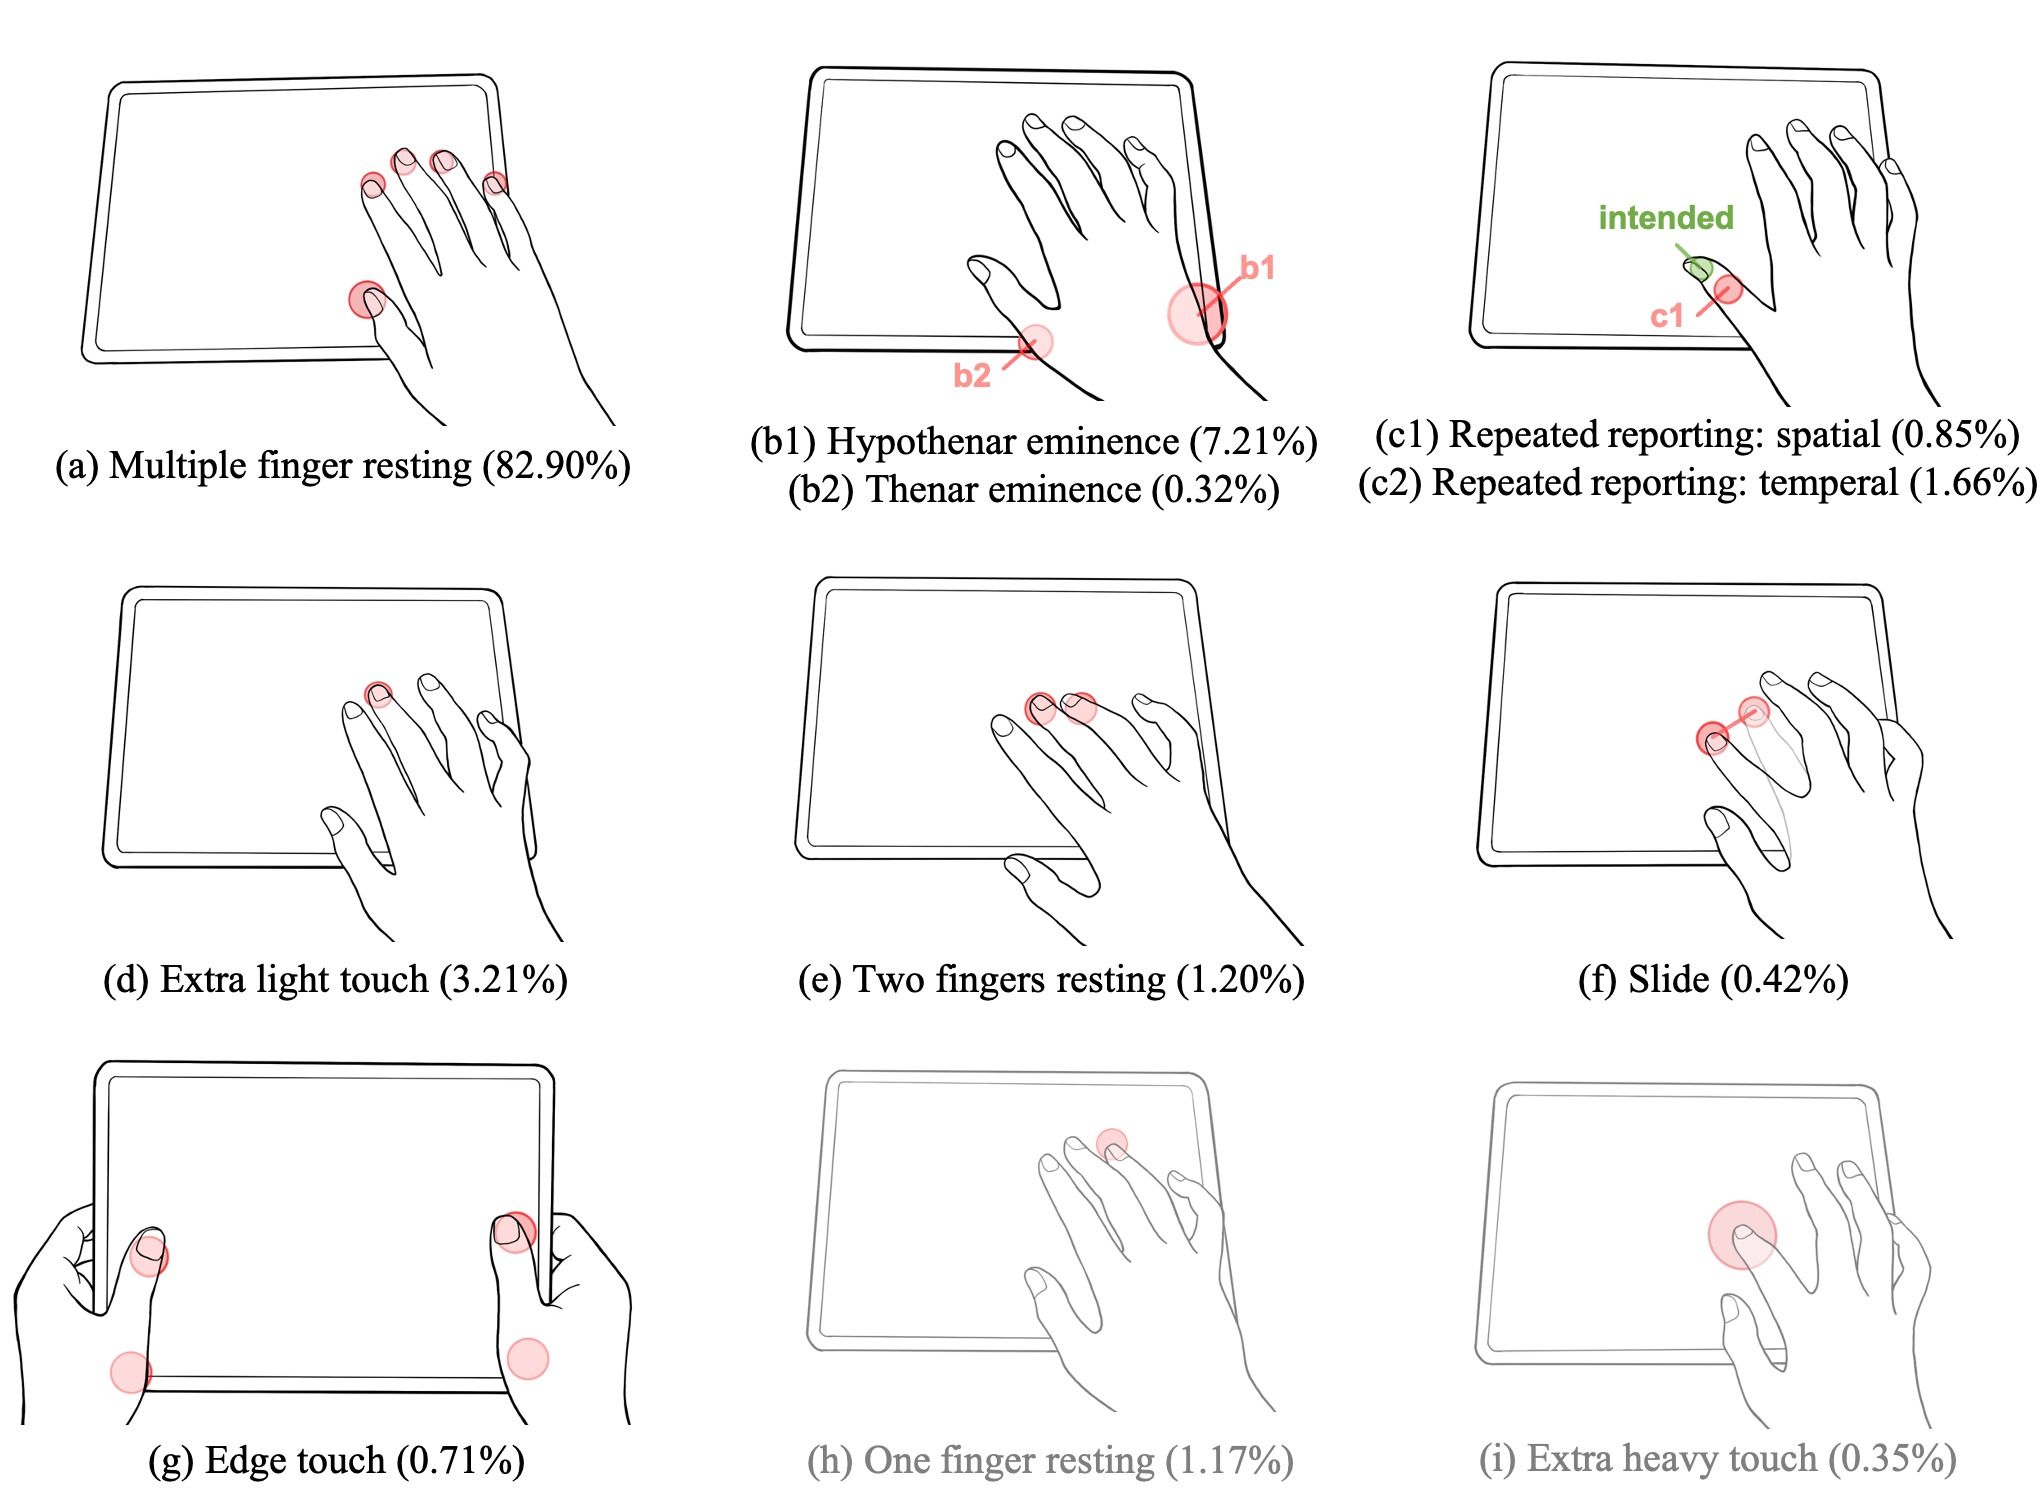
\includegraphics[width=1.0\linewidth]{figures/TypeBoard_unintentional_touch.png}
	\centering
	\caption*{图中展示了所有的九种误触的情形,其中括号中的数值是该类型误触占所有误触的比例。}
	\caption{所有的误触类型图示}
	\label{fig:TypeBoard_unintentional_touch}
\end{figure}

\subsection{关于防误触键盘的讨论}

\subsubsection{与先前工作的对比}

TapBoard\cite{2013-TapBoard}是与本章最类似的相关工作,请注意本章所介绍的TypeBoard与TapBoard是不同的,这两份工作都探讨了触摸屏键盘上的误触问题。然而,先前工作TapBoard存在两个致命缺陷:首先,TapBoard强行将敲击手势定为有意触摸,将其它触摸手势定为误触,其中敲击手势指的是位移小于15毫米、触摸时长短于450毫秒的触摸。这种要求人去适应技术的设计违反了人机交互的自然性原则。第二,TapBoard只能在触摸的手指抬起时判断触摸的有意性,响应性比正常的键盘低,尽管如此,其识别准确率也只有97\%。当实验者复现TapBoard技术,并将其应用于本节实验所采集的自然打字行为数据集上时,TapBoard的误触识别准确率仅为73.83\%(SD=14.39\%),这一表现远低于本章所介绍的防误触技术TypeBoard(98.88\%, SD = 0.73\%)。以上对比表明,本章所介绍的防误触技术显著优于先前技术。

\subsubsection{用户差异}

如图\ref{fig:TypeBoard_u_touches_over_user_task}(左侧)所示,不同被试的打字行为有较大差异。举一些极端的例子,被试P1平均每100次有意触摸就会产生74.40次无意触摸,而被试P16在整个实验过程中仅产生了三次无意触摸。实验者按被试的心理将他们分为三类:(1)P1-P10属于第一类被试,他们愿意在打字的过程中将非交互手指休息在触摸屏上,因此会产生大量的无意触摸。(2)P11-P12属于第二类被试,他们相信TypeBoard能够防止误触,放心地将手掌休息在触摸屏的边缘,但很少将非交互手指休息在触摸屏上。系统为这部分被试过滤了大量的边缘误触。P12评论道:“\emph{我不会将手指休息在触摸屏上,因为已经在触摸屏上的手指无法像在物理键盘上一样直接按下去。}”(3)P13-P16在打字过程中时刻将双手悬空,他们在TypeBoard上打字的行为和在普通平板电脑上打字的行为并无太大差别,说明他们并未主动尝试TypeBoard防误触键盘带来的新体验。P13-P16在平板电脑键盘上的打字经验差异很大,P13和P14在平板电脑上打字经验仅为一年,P15没有相关经验。P16是平板电脑打字的专家用户,他几乎不产生任何无意触摸,这是因为他在普通的平板电脑键盘上也能盲打。上述分析说明,用户个性化对于本章介绍的防误触键盘技术来说是很有价值的。

\begin{figure}[!tbh]
	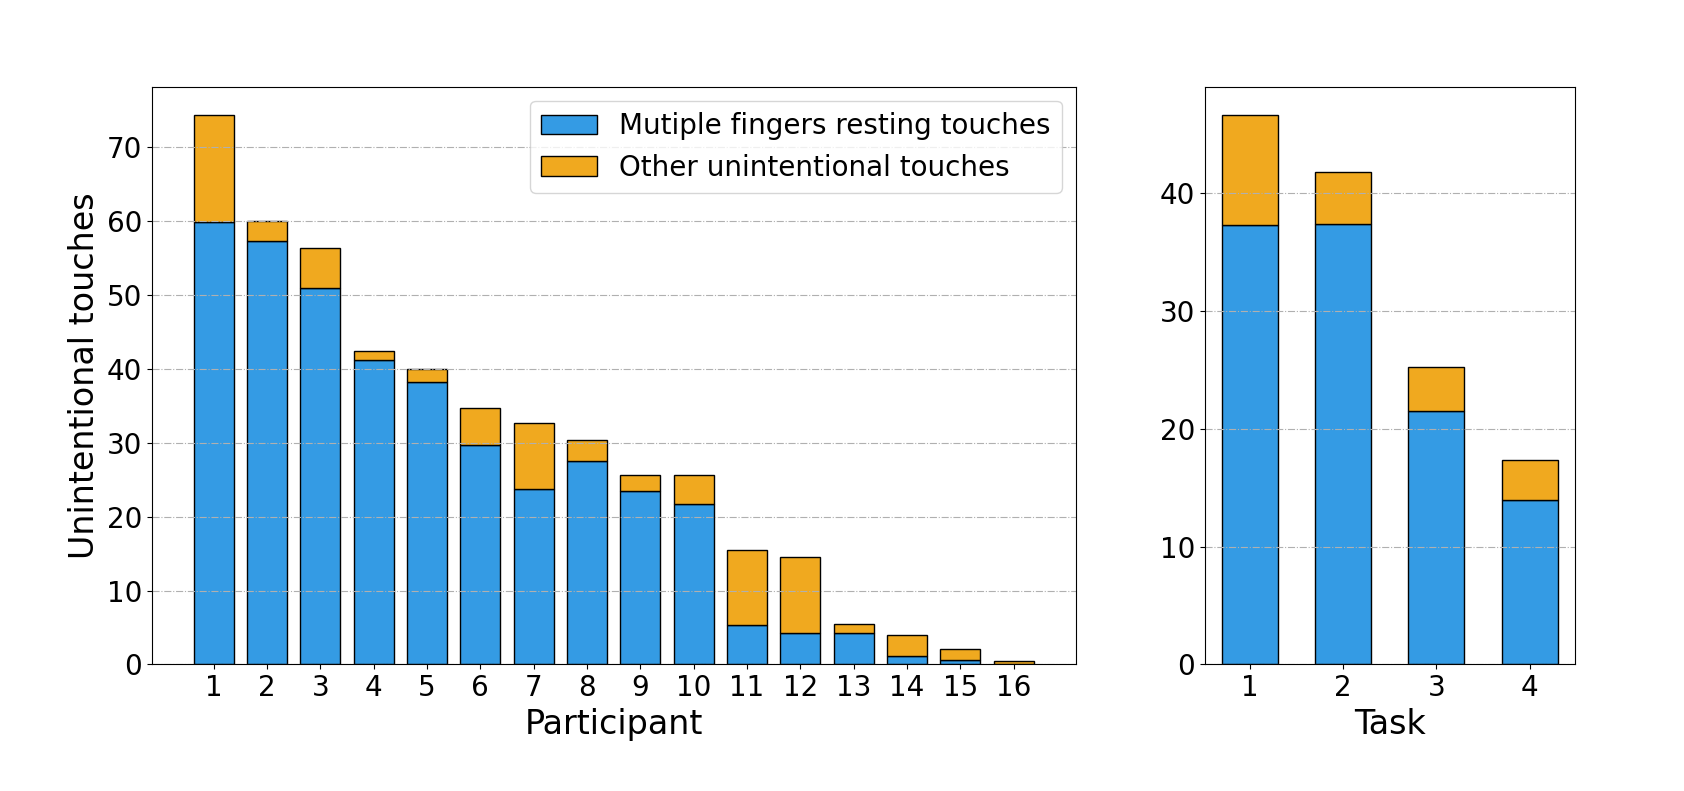
\includegraphics[width=1.0\linewidth]{figures/TypeBoard_u_touches_over_user_task.png}
	\centering
	\caption*{左图是不同被试在无意触摸计数上的差异,右图是不同任务在无意触摸计数上的差异。}
	\caption{用户差异和任务差异图示}
	\label{fig:TypeBoard_u_touches_over_user_task}
\end{figure}

\subsubsection{任务差异}

如图\ref{fig:TypeBoard_u_touches_over_user_task}(右侧)所示,不同文本输入任务下无意触摸的数量有较大差异。在四个不同的实验任务下,被试平均每100次触摸会产生46.67次(SD=48.01)、41.78次(SD=52.65)、25.28次(SD=37.82)和17.37次(SD=14.50)无意触摸。匹配样本T检验显示以下实验任务之间,多指休息导致的无意触摸数量存在显著性差异:1-3($t_{15}=2.58,p<.05$)、1-4($t_{15}=2.23,p<.05$)。被试在第四个实验任务中更少地将手指休息在触摸板上,这是因为第四个任务看图写话不需要频繁切换文本输入和光标控制。结果表明,文本输入任务的多样性对误触研究来说是十分重要的,然而,这一多样性在相关文献中往往被忽视\cite{2013-TapBoard, 2020-TabletopTouch, 2014-PalmRejection}。

\subsubsection{为什么要采样100毫秒的数据来判别误触?} 

数据采用的时间越长,有用的信息越多,对误触的判别准确率也会越高。然而,太长的采样时间又会导致较大的延迟,影响用户体验。因此,技术的识别准确率和延迟之间存在权衡的问题。为了找到一个好的平衡点,实验者通过模拟实验评测了不同延迟下误触识别准确率的变化,结果如图\ref{fig:TypeBoard_error_rate_diss}(左侧)所示。重复测量方差分析显示延迟对误触识别准确率有显著影响($F_{4,56}=4.88, p<0.05$),后验测试显示以下延迟对之间存在显著差异:60毫秒-100毫秒(p<.05)、60毫秒-120毫秒(p<.05)、60毫秒-140毫秒(p<.05)、80毫秒-140毫秒(p<.05)。也就是说,当延迟超过100毫秒时,延迟的进一步增长不再带来准确率的提高。因此,100毫秒的识别延迟是最佳选择,使得误触识别的准确率达到98.88\%。触摸交互中100毫秒的延迟是用户可察觉的,但不会显著影响用户的交互效率\cite{2017-System, 2014-Towards, 2016-Latency}。

\begin{figure}[!tbh]
	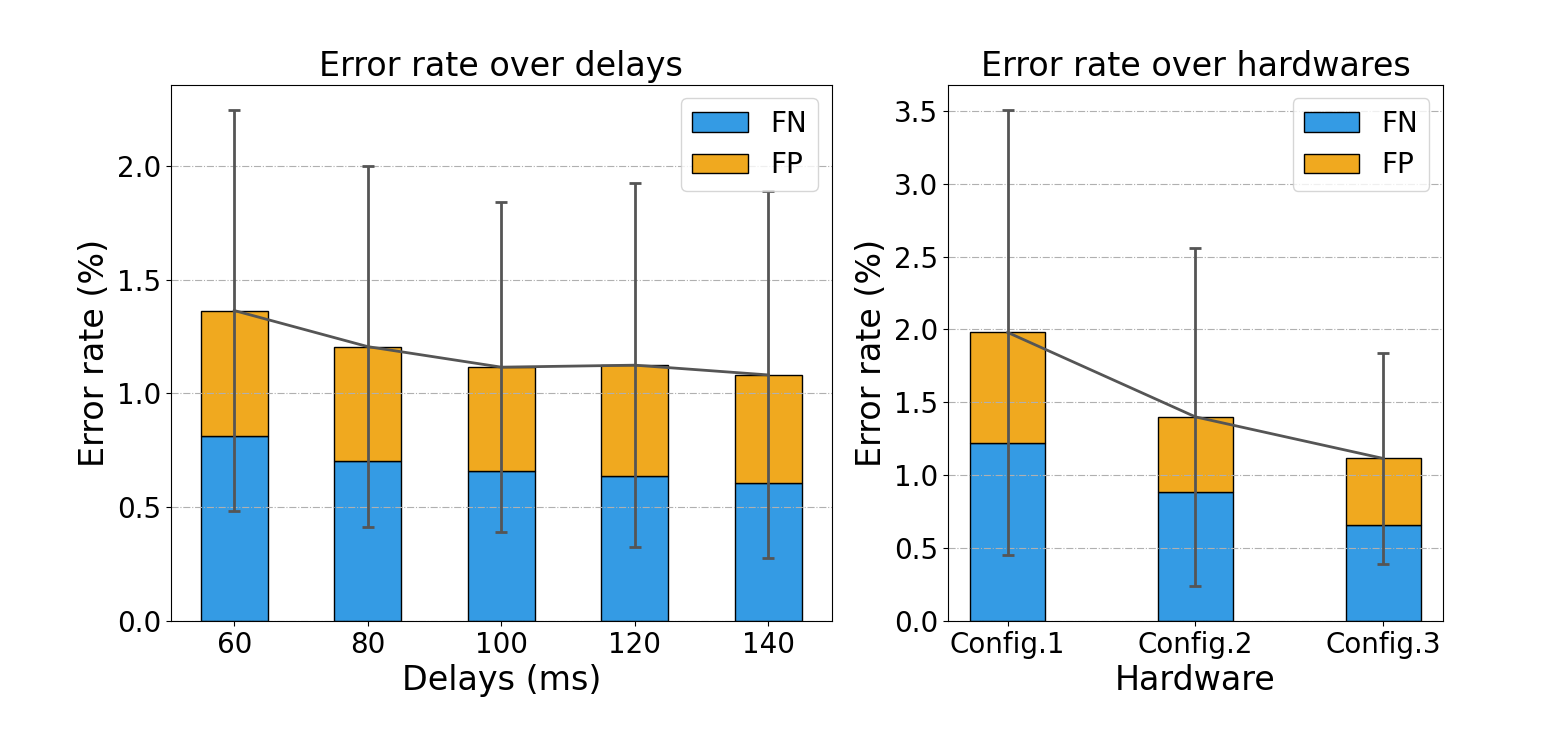
\includegraphics[width=1.0\linewidth]{figures/TypeBoard_error_rate_diss.png}
	\centering
	\caption*{左图展示了不同信号采集时间下误触识别的准确率,右图展示了不同信号组合下误触识别的准确率。}
	\caption{采样时间和信道对误触识别准确率的影响}
	\label{fig:TypeBoard_error_rate_diss}
\end{figure}

\subsubsection{本技术是否适用于更少的传感器?}

本章的各种实验数据已经证明,压敏触摸板上的压力信号对误触识别的准确率来说是至关重要的。然而,目前市面上大多数触摸屏设备都不具备全屏幕压力传感的能力,而小部分设备(如MacBook触摸板)能够传感触摸板受到的总压力。为了探索本技术是否适用于更少的传感器,实验者通过数据模拟分析了三种硬件设置下本防误触技术的表现。

\begin{enumerate}
	\item \textbf{电容触摸屏}:最常用的电容式触摸屏设备仅能提供电容屏信号,而不能提供任何压力相关的信号。为了评测本防误触技术在电容式触摸屏上的表现,实验者删除了支持向量机模型所用特征向量中所有和压力信号有关系的特征,并重新训练模型。
	\item \textbf{压力触摸板}:苹果电脑的压力触摸板可以用四个角上的压力传感器计算触摸板所受到的总压力。为了评测本防误触技术在压力触摸板上的表现,实验者将特征向量中涉及到的触点压力信号用估算值来代替,触点压力的估算方法是用总压力乘以该触点的接触面积占所有触点接触面积之和的比例。
	\item \textbf{压敏触摸板}:本实验中用到的设备即为压敏触摸板,能够直接测量每个触点的压力。
\end{enumerate}

如图\ref{fig:TypeBoard_error_rate_diss}(右侧)所示是本防误触技术在上述三种硬件设置下的误触识别率。重复测量方差分析现实硬件设置对误触识别的准确率有显著性影响($F_{2,28}=10.52, p<0.001$)。Bonferroni校正后验测试显示以下硬件设置对之间存在显著性差异:1-2(p<.005)、1-3(p<.005)。设置2和设置3之间的准确率差异仅为趋势(p=.062)。这一结果表明,本防误触技术在压敏触摸板上的表现最佳;而在只能识别总压力的压力触摸板上表现也不错,压力触摸板是性价比很高的选择。

\subsubsection{迭代方法}

由于技术会影响用户行为,而数据驱动的技术在研发过程中又需要先采集用户行为数据,所以数据驱动的技术和用户行为之间存在死锁问题。本章工作提出了解决上述死锁问题的迭代方法,即实验者首先研发了初版防误触技术,采集用户在初版防误触键盘上的打字行为数据,最后根据行为数据研发终版防误触技术。相比之下,大多数先前研究都在无反馈的情况下(类似本章的实验一)收集用户的行为数据\cite{matero2012identifying, 2014-PenMightier, 2018-PalmTouch},或者在替代性反馈下收集数据\cite{2013-TapBoard, 2020-TabletopTouch},以回避死锁问题。作者认为本章所述的迭代方法值得更多的关注,在本章所介绍的工作中,实验二采集到的数据和实验一数据之间存在较大差异,也就是说,迭代的方法能够得到更接近真实的用户行为数据,而基于更真实数据的交互技术也会更能理解人的交互意图。

\subsubsection{为什么不采用深度学习?}

本章使用经典的机器学习方法(支持向量机)来解决防误触问题,而没有用到深度学习,这是因为,防误触技术作为触摸屏设备的一项底层技术,需要速度快、功耗低的解决方案。深度学习是一种计算密集型的算法,并不满足防误触技术的要求。出于这个原因,作者认为经典的机器学习方法更适用于本技术。

\subsubsection{提高防误触能力其它方法}

首先,可以利用触点与键盘布局之间的关系辅助对触点有意性的判断,例如,当触点没有落在任何按钮上上,它更有可能是一次误触。第二,可以使用语音模型作为先验知识。贝叶斯解码器被广泛应用于从词汇表中预测用户所需的单词\cite{gong2018wristext, gordon2016watchwriter, gupta2019rotoswype, markussen2014vulture}。贝叶斯解码器还可以用于计算后续触摸点落在不同位置上的概率分布,当触摸落在低概率的按键上时,它更有可能是误触。在本章介绍的防误触技术当中,实验者没有将键盘布局和语言模型作为先验知识,因为本章所探索的是面向平板电脑键盘的通用的防误触方法。

\section{防误触键盘的评测}

\subsection{实验三:防误触键盘的评测实验}

实验三的目的有两点:首先,实验三比较了平板电脑上防误触键盘TypeBoard和普通软键盘的文本输入效率;第二,如本章引言所述,若在防误触键盘上加上按键的轮廓反馈,将能大大提升文本输入效率,因此实验三还评测了TypeBoard+的表现,TypeBoard+即为加上了按键轮廓反馈的防误触键盘。总的来说,本实验比较了被试在三种平板电脑键盘上的打字效率和用户体验:(1)普通触摸屏键盘;(2)TypeBoard;(3)TypeBoard+。

\subsubsection{被试}

实验者从校园中招募了15名被试参与实验,被试的年龄从19岁到26岁不等,平均年龄为20.87岁,标准差为2.42,其中有7名女性被试。所有被试都是右撇子,他们没有参与过之前的用户实验。被试们拥有不少于两年的智能手机打字经验,平均经验为6.67年,标准差为2.06。11名被试有平板电脑十指打字经验。

\subsubsection{实验设计和过程}

本实验采用了组内实验设计,即每名被试都会使用三种不同的键盘进行实验。被试坐在一张可以调节高度的座椅上,他们可以将座椅调整至舒适的高度。被试们在一块压敏触摸板上打字,在平板电脑上获取视觉反馈。如图\ref{fig:TypeBoard_study3_illu}所示,实验涉及到三种键盘设置:

\begin{enumerate}
	\item \textbf{设置一}:\emph{普通键盘}。在普通的平板电脑文本输入中,触摸板上所有的触摸都会被视为有意交互,被试在打字过程中需要双手悬空,或者将手腕休息在触摸板外,以避免误触。
	\item \textbf{设置二}:\emph{TypeBoard}。实验二中所介绍的平板电脑防误触键盘,键盘只会对它认为的有意触摸做出响应,被试在打字过程中可以将非交互手指休息在触摸板上。
	\item \textbf{设置三}:\emph{TypeBoard+}。在防误触键盘的基础上,加上按键轮廓的触觉反馈。为了提供触觉反馈,实验者在每个按键上贴上了0.05毫米厚的贴纸,在F键和J键上有额外的凸起,这一凸起的设置和物理键盘一样。被试可以通过触摸贴纸的边缘来定位自己的手指,从而有机会实现盲打。
\end{enumerate}

\begin{figure}[!tbh]
	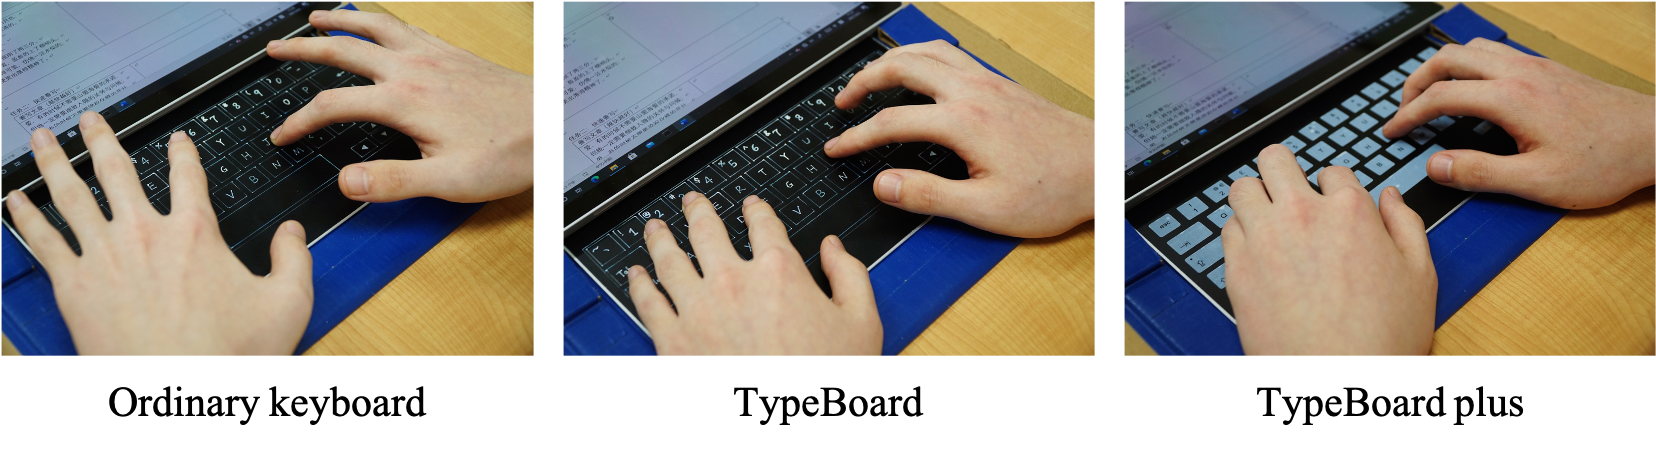
\includegraphics[width=1.0\linewidth]{figures/TypeBoard_study3_illu.png}
	\centering
	\caption*{从左到右三幅子图分别表示实验三}
	\caption{实验三的实验设置}
	\label{fig:TypeBoard_study3_illu}
\end{figure}

在每种键盘设置下,有五段重复实验,每段实验被试誊写一段中文文字。誊写是文本输入研究中最常用的实验任务\cite{2003-Metrics, mackenzie2003phrase, 2017-Word},一般用于评测文本输入法的打字效率上限。每段中文文本大约包含100个字,这些文本段落是从一个打字测速网站\cite{Website-Typing}中随机抽选的。被试需要尽可能又快又准地完成文本输入实验。实验采用拉丁方来平衡三种键盘设置的出场顺序。在每一种键盘设置的正式实验开始前,被试有五分钟的热身时间通过誊写文本来熟悉键盘的设置,热身过程中用过的文本不会出现在正式实验中。在每两段实验之间,被试休息两分钟的时间以避免疲劳。平均而言,本实验的总时长为90分钟。

\subsection{防误触键盘的评测结果}

实验者使用重复测量方差分析来评估组内因素键盘设置对打字速度、未纠正错误率(UER)和已纠正错误率(CER)的显著性影响。由于UER和CER不服从正态分布,实验者在方差分析之前使用对齐秩变换算法\cite{2011-Aligned}校准数据。如果有任何独立变量对实验结果有显著性影响(p<.05),实验者采用Bonferroni校正后的后验测试来做成对比较。

\subsubsection{打字速度}

本节将用每分钟输入中文字个数(CPM)来测量被试的打字速度:

\begin{equation}
	CPM = \frac{|S|}{T} \times 60
\end{equation}

其中,|S|是所誊写的中文文本的长度(包括标点符号),T是被试完成输入的时间,即从第一次有意触摸到最后一次有意触摸之间所用的时间。

\begin{figure}[!tbh]
 	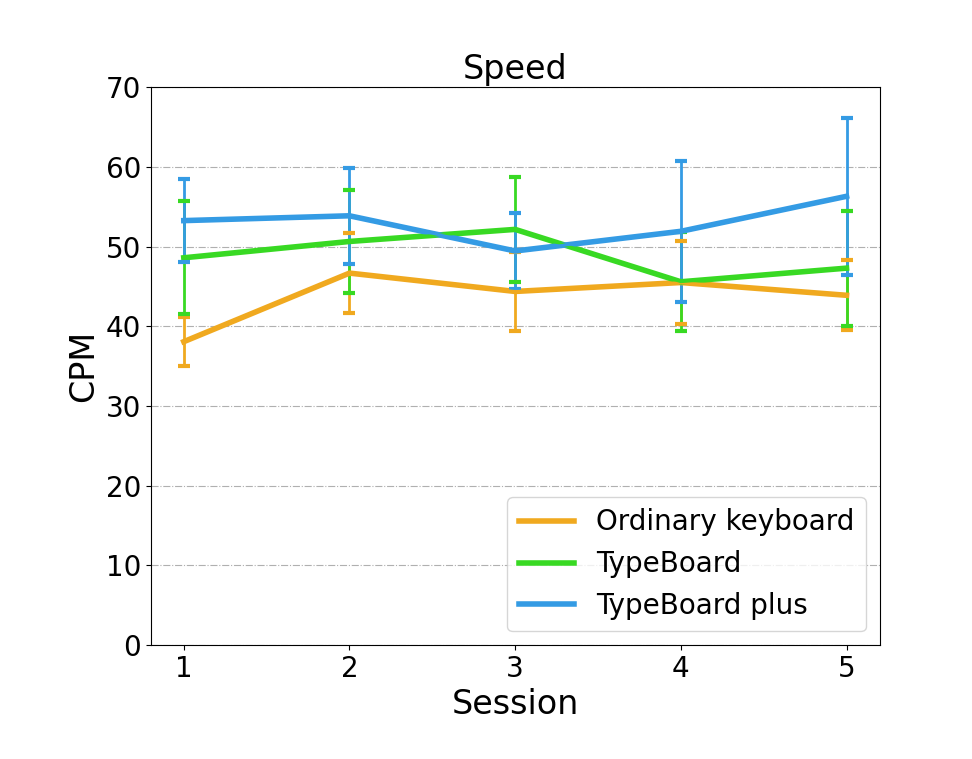
\includegraphics[width=0.7\linewidth]{figures/TypeBoard_speed.png}
	\centering
	\caption*{图中展示了三种不同键盘设置下,被试的打字速度随着实验时间推移二变化的折线图,误差条表示95\%置信区间。}
	\caption{三种键盘下被试打字速度对比}
	\label{fig:TypeBoard_speed}
\end{figure}

如图\ref{fig:TypeBoard_speed}所示是被试的打字速度随着实验段数变化的折线图。实验段数对打字速度没有显著性影响($F_{4,56}=1.76,p=.15$),结果表明,这三款平板电脑键盘的学习成本很低,用户刚上手就能达到可观的文本输入速度。键盘设置对打字速度有显著影响($F_{2,28}=26.76,p<.001$),成对比较显示,所有的键盘设置之间都存在显著差异:普通键盘-TypeBoard($p<.005$)、普通键盘-TypeBoard+($p<.001$)、TypeBoard-TypeBoard+($p<.005$)。被试在普通键盘上的平均打字速度为43.71 CPM(SD=6.52),在TypeBoard上的打字速度为48.87 CPM(SD=10.14),超出普通键盘打字效率11.78\%。被试在TypeBoard+上的打字速度为52.97 CPM(SD=9.85),超出普通键盘打字效率21.19\%。结果表明,面向平板电脑文本输入的防误触技术大幅度提高了打字效率。

为了比较TypeBoard+和物理键盘,实验者组织了一次非正式实验测量了实验三被试在物理键盘上的打字速度。被试们通过自己熟悉的物理键盘在一个中文打字测速网站上输入五段文字\cite{Website-Typing},平均速度达到65.01 CPM(SD=9.26)。这一结果表明,TypeBoard+和物理键盘之间还是有一定差距的,但是和普通平板电脑键盘相比,这一差距已经缩小了43.48\%。

\subsubsection{打字错误率}

本节用两种指标来评测文本输入法的错误率:(1)未纠正错误率(UER)——遗留在所誊写文本中的错误,UER等于为未经纠错的中文字个数除以所誊写句子的字数;(2)已纠正错误率(CER)——那些在打字过程中被纠正(例如通过删除)的错误,CER等于被纠正的中文字个数除以誊写句子的字数。被试使用拼音输入法过程中对字母的纠正未算入CER指标中。由于UER和CER不服从正态分布,实验者使用对齐秩变换算法\cite{2011-Aligned}校正数据。

\begin{figure}[!tbh]
	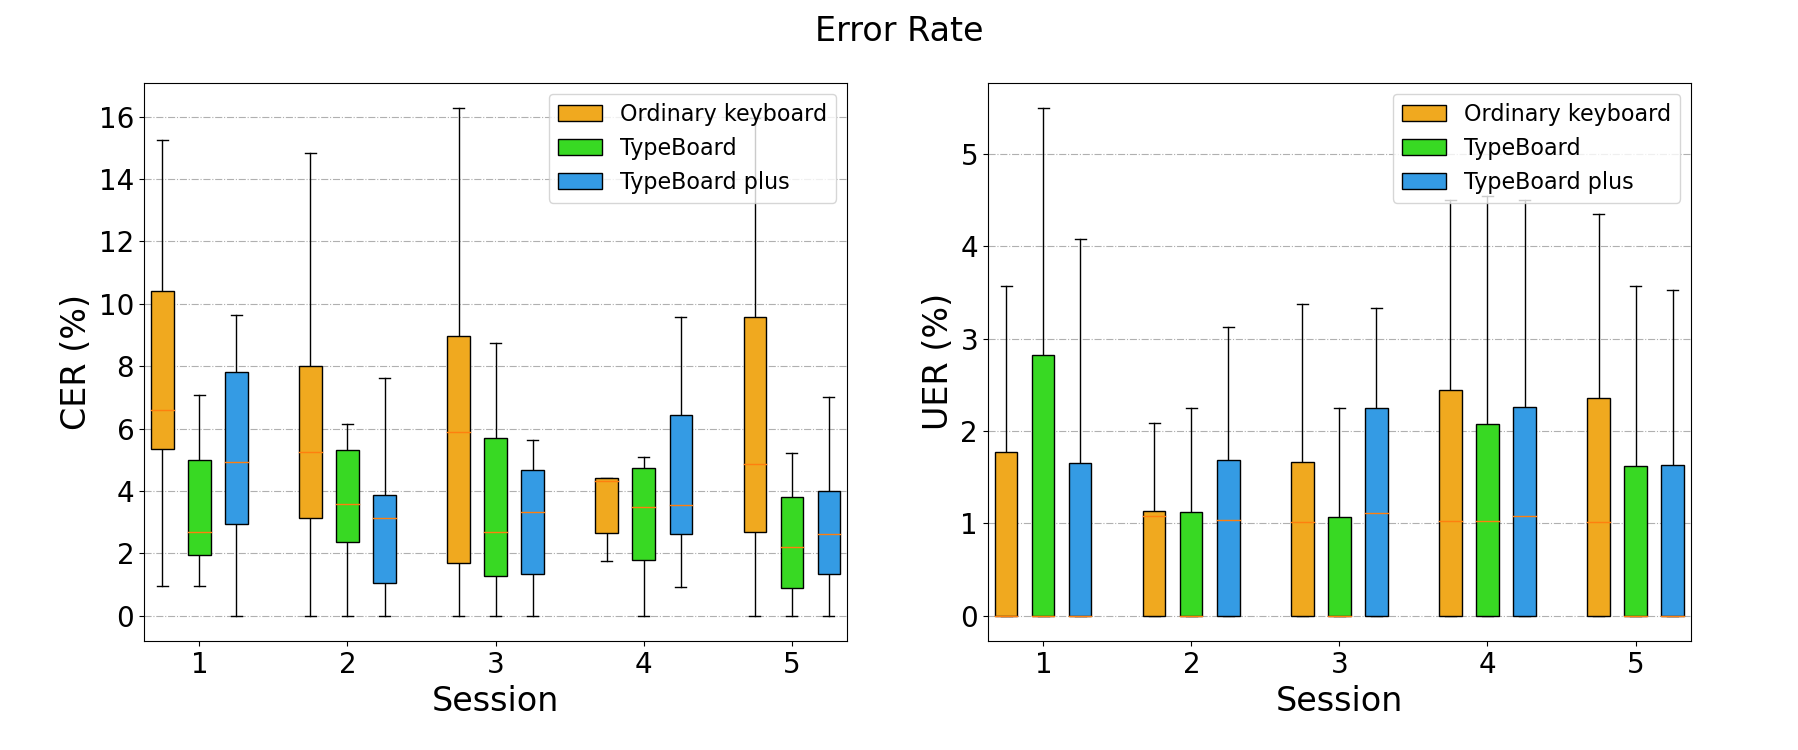
\includegraphics[width=1.0\linewidth]{figures/TypeBoard_error_rate.png}
	\centering
	\caption*{图中展示了三种键盘设置下,已纠正错误率和未纠正错误率的箱型图。}
	\caption{打字错误率图示}
	\label{fig:TypeBoard_error_rate}
\end{figure}

如图\ref{fig:TypeBoard_error_rate}所示是已纠正错误率(CER)和未纠正错误率(UER)随实验段数变化的箱型图。实验段数对CER没有显著影响($F_{4,56}=1.01,p=.39$),键盘设置对CER有显著影响($F_{2,28}=9.49,p<.005$),后验测试显示以下键盘设置的CER之间存在显著差异:普通键盘-TypeBoard($p<.01$)、普通键盘-TypeBoard+($p<.005$)。普通键盘、TypeBoard和TypeBoard+下的平均CER分别是6.66\%(SD=4.42\%)、4.58\%(SD=3.58\%)和4.21\%(SD=2.58\%)。实验段数($F_{4,56}=0.41,p=.71$)和键盘设置($F_{2,28}=0.001,p=.998$)都对UER没有显著影响。普通键盘、TypeBoard和TypeBoard+下的平均UER分别是1.29\%(SD=1.67\%)、1.28\%(SD=1.38\%)和1.28\%(SD=1.16\%)。结果表明,防误触技术降低了用户在平板电脑触摸屏上打字时打错字的概率,这是TypeBoard提高了平板电脑打字速度的主要原因。与TypeBoard相比,TypeBoard+在降低打字错误率上没有显著的优势,这说明TypeBoard+的打字效率更高是另有原因的。

\subsubsection{时间构成}

为了深入探讨本技术的用户打字效率问题,实验者将被试的文本输入耗时拆分成三个构成部分:键入时间、选词时间和停顿时间。键入时间指的是被试点击单词各个字母所用的时间,是从被试点击单词首字母到点击单词尾字母之间的时间。选词时间是被试从候选词列表中选中所需单词的时间。停顿时间是从完成一个单词的选词到输入下一个单词首字母所需的时间。上述时间指的都是每输入一个英文单词所消耗的时间。

为了深入探讨三种键盘设置对用户打字效率和体验的影响,实验者将被试的文本输入耗时拆分成四个构成部分:键入时间、选词时间、删除时间和停顿时间。键入时间是被试点选拼音中每个字母所用的时间,是从被试点击拼音首字母到点击拼音尾字母之间的时间。选词时间是被试从拼音输入法中选择所需中文字或词所用的时间。删除时间是删除拼音或中文字所需的时间。停顿时间是从完成一个中文字或词到输入下一个拼音首字母所需的时间。如图\ref{fig:TypeBoard_time_components}所示是每输入一个中文字所消耗的键入时间、选词时间、删除时间和停顿时间。重复测量方差分析显示键盘设置对选词时间($F_{2,28}=7.85,p<.005$)、删除时间($F_{2,28}=20.89,p<.001$)和停顿时间($F_{2,28}=12.76,p<.001$)都有显著影响。后验测试显示TypeBoard($p<.001$)和TypeBoard+($p<.001$)都与普通键盘相比都能显著降低删除时间,这一结果表明,防误触键盘技术降低了打字的错误率。TypeBoard+在停顿时间上显著优于普通键盘($p<.001$)和TypeBoard($p<.005$),这一结果表明TypeBoard+上的按键轮廓反馈让用户有机会实现盲打,省去了键入新字时目光在任务文本和键盘之间来回切换的时间。

\begin{figure}[!tbh]
	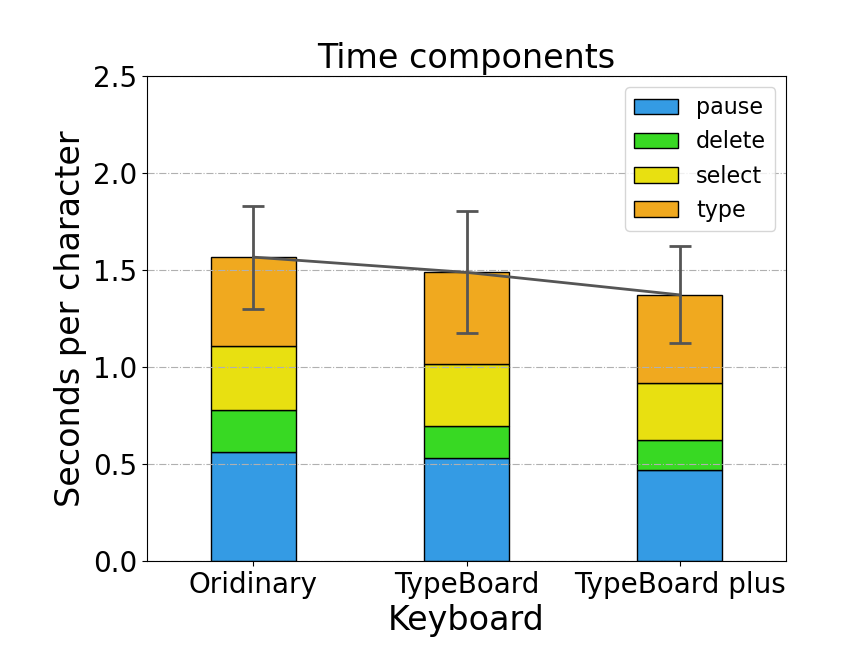
\includegraphics[width=0.7\linewidth]{figures/TypeBoard_time_components.png}
	\centering
	\caption*{图中展示了被试每输入一个中文字时各个动作所消耗的时间,误差条表示95\%置信区间}
	\caption{时间构成}
	\label{fig:TypeBoard_time_components}
\end{figure}

\subsubsection{触点位置}

如图\ref{fig:TypeBoard_touch_position}所示分别是TypeBoard和TypeBoard+下有意触摸位置的点云分布。为了方便观察,实验者默认点云符合二维高斯分布。实验中键盘每个按键的宽度为17毫米,TypeBoard上触摸点云中心点位置与键盘中心位置之间在X轴/Y轴上的偏移量分别为-1.03/-0.29毫米,TypeBoard+上偏移量为-2.02/-0.59毫米。这一偏移量相对于按键宽度来说是很小的,说明被试的触摸点击非常接近每个按键的中心。TypeBoard上触摸点云在X轴/Y轴上的标准差分别为5.66/5.07毫米,TypeBoard+上标准差为5.01/4.53毫米。成对采样T检验显示,键盘设置对触摸点云的在两个轴上标准差之积存在显著影响($t_{15}=-4.65,p<.001$),这一结果表明,被试在TypeBoard+上的触摸行为更加精准,TypeBoard+上的按键轮廓反馈有助于提高用户触摸行为的精准性,从而提高打字效率。

\begin{figure}[!tbh]
	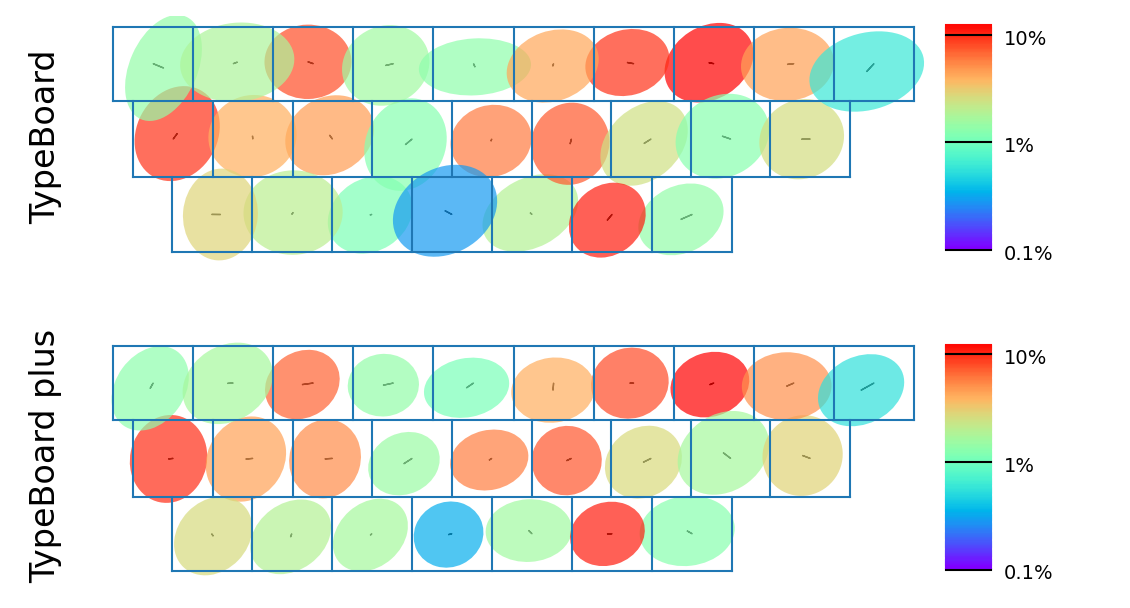
\includegraphics[width=1.0\linewidth]{figures/TypeBoard_touch_position.png}
	\centering
	\caption*{上图展示了TypeBoard下触摸点云的分布图,下图展示了TypeBoard+的点云图。椭圆表示二维高斯分布的三倍标准差的范围。热度图表示每个字母被点击的频率。}
	\caption{两种键盘的触摸点云图示}
	\label{fig:TypeBoard_touch_position}
\end{figure}

\subsubsection{主观评分}

被试在实验结束后,通过7级李克特量表为三种键盘的主观打字速度、打字准确率、疲劳程度和认知负担打分(1分最差,7分最佳)。如图\ref{fig:TypeBoard_subjective_feedback}所示是主观评分的结果。Wilcoxon Signed-Rank测试表明TypeBoard显著提升了平板电脑键盘的主观打字速度($Z=-2.27,p<.05$)、打字准确率($Z=-3.24,p<.005$),降低了疲劳感($Z=-2.84,p<.005$)和认知负担($Z=-1.99,p<.05$)。TypeBoard+也显著提升了平板电脑键盘的主观打字速度($Z=-3.17,p<.005$)、打字准确率($Z=-3.52,p<.001$),降低了疲劳感($Z=-3.34,p<.001$)和认知负担($Z=-2.28,p<.05$)。TypeBoard+在主观打字速度($Z=-2.40,p<.05$)和疲劳感($Z=-2.85,p<.005$)上比TypeBoard更优。结果表明TypeBoard和TypeBoard+都优化了平板电脑触摸屏打字的用户体验。

\begin{figure}[!tbh]
	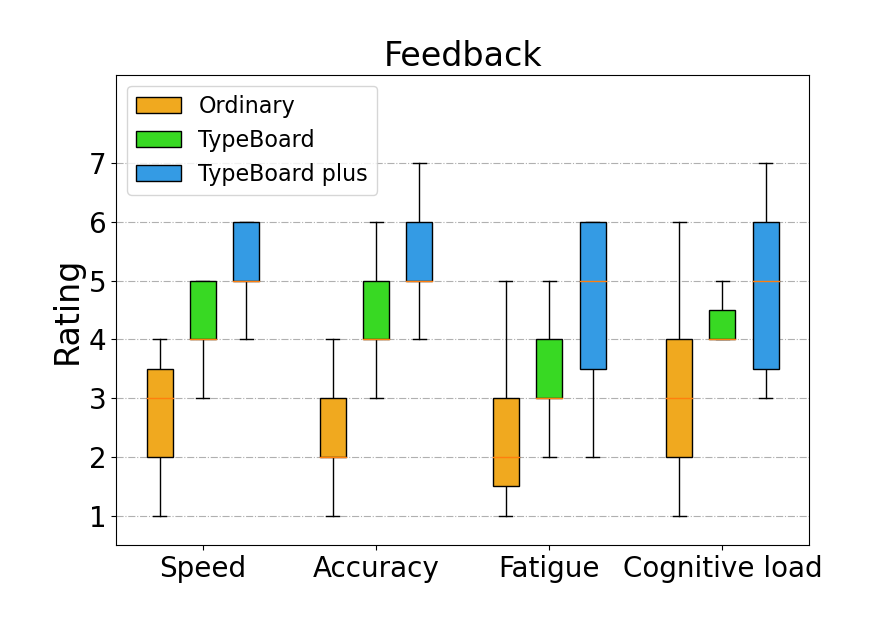
\includegraphics[width=0.7\linewidth]{figures/TypeBoard_subjective_feedback.png}
	\centering
	\caption*{图中展示了三种键盘设置下被试的主观打字速度、打字准确率、疲劳程度和认知负担打分(1分最差,7分最佳)。}
	\caption{主观评分}
	\label{fig:TypeBoard_subjective_feedback}
\end{figure}

\subsubsection{实验结果小结}

(1)与平板电脑触摸屏上的普通键盘相比,TypeBoard防误触技术将打字效率提高了11.78\%。具有缓解疲劳、降低认知负担和减少打字错误率的好处。(2)TypeBoard+进一步将TypeBoard的打字效率提升8.51\%,与普通键盘相比提高了21.19\%。TypeBoard+的优点是提高用户打字行为的精准性和减少打字过程中寻找按键的时间。结果表明,本触摸屏防误触技术提高了文本输入技术的效率和用户体验,也为触摸屏上的盲打体验奠定了基础。

\section{本章小结}

本章介绍了面向平板电脑文本输入的防误触技术(TypeBoard),它可以过滤98.88\%的误触。该技术强大的防误触能力改变了用户在平板电脑上打字的行为习惯,使得用户在平板电脑上打字时愿意将非交互手指休息在触摸屏上,以避免长时间打字带来的疲劳。平均而言,用户在TypeBoard上每100次有意触摸就会产生40.83次无意触摸,大部分都被该防误触技术过滤了。评测实验发现,防误触技术将平板电脑上的文本输入效率提高了11.78\%。在用户可以将手指休息在触摸屏上,而不引发误触的前提下,实验者在触摸屏上加上了键盘按键的轮廓反馈,使得用户可以在触摸屏上盲打,这进一步将平板电脑上的文本输入效率提高到原来的21.18\%。结果显示,防误触技术在诸多方面提升了平板电脑文本输入法的效率和用户体验,包括缓解疲劳、降低打字错误率和间接支持了触摸屏盲打。
